%----------------------------------------------------------------------------------------
%	PACKAGES AND THEMES
%----------------------------------------------------------------------------------------


\documentclass{beamer}

\mode<presentation> {

% The Beamer class comes with a number of default slide themes
% which change the colors and layouts of slides. Below this is a list
% of all the themes, uncomment each in turn to see what they look like.


\usepackage{qtree}
\usepackage{amsthm}
\usepackage{algpseudocode}
\usepackage[export]{adjustbox}
\usepackage{subcaption}
\usepackage{hyperref}
\usepackage{graphicx}
\usepackage{tabularx}
\usepackage{mdframed}
\usepackage{framed}
\usepackage{siunitx}
\usepackage{placeins}
\usepackage{units}
\usepackage{xcolor}
\usepackage{lipsum}
\usepackage{algorithm}
\usepackage{amsmath}
\usepackage{paralist}
\usepackage{mdwlist}
\usepackage[labeled]{multibib}
\usepackage{array}
\usepackage{newfloat}
\usepackage{datetime}

%\usetheme{default}
%\usetheme{AnnArbor}
%\usetheme{Antibes}
%\usetheme{Bergen}
%\usetheme{Berkeley}
%\usetheme{Berlin}
%\usetheme{Boadilla}
%\usetheme{CambridgeUS}
%\usetheme{Copenhagen}
%\usetheme{Darmstadt}
%\usetheme{Dresden}
%\usetheme{Frankfurt}
%\usetheme{Goettingen}
%\usetheme{Hannover}
%\usetheme{Ilmenau}
%\usetheme{JuanLesPins}

%\usetheme{Luebeck}
\usetheme{Madrid}
%\usetheme{Malmoe}
%\usetheme{Marburg}
%\usetheme{Montpellier}
%\usetheme{PaloAlto}
%\usetheme{Pittsburgh}
%\usetheme{Rochester}
%\usetheme{Singapore}
%\usetheme{Szeged}
%\usetheme{Warsaw}

% As well as themes, the Beamer class has a number of color themes
% for any slide theme. Uncomment each of these in turn to see how it
% changes the colors of your current slide theme.

%\usecolortheme{albatross}
%\usecolortheme{beaver}
%\usecolortheme{beetle}
%\usecolortheme{crane}
%\usecolortheme{dolphin}
%\usecolortheme{dove}
%\usecolortheme{fly}
%\usecolortheme{lily}
%\usecolortheme{orchid}
%\usecolortheme{rose}
%\usecolortheme{seagull}
%\usecolortheme{seahorse}
%\usecolortheme{whale}
%\usecolortheme{wolverine}

%\setbeamertemplate{footline} % To remove the footer line in all slides uncomment this line
%\setbeamertemplate{footline}[page number] % To replace the footer line in all slides with a simple slide count uncomment this line

%\setbeamertemplate{navigation symbols}{} % To remove the navigation symbols from the bottom of all slides uncomment this line
}

\usepackage{graphicx} % Allows including images
\usepackage{booktabs} % Allows the use of \toprule, \midrule and \bottomrule in tables

%----------------------------------------------------------------------------------------
%	TITLE PAGE
%----------------------------------------------------------------------------------------

\title[Wavelet Tree]{Engineering Rank and Select Queries on Wavelet Trees} % The short title appears at the bottom of every slide, the full title is only on the title page

\author{Roland Larsen Pedersen} % Your name
\institute[Datalogi] % Your institution as it will appear on the bottom of every slide, may be shorthand to save space
{
Datalogi, Aarhus Universitet \\ % Your institution for the title page
\medskip
\textit{Thesis defence}
}
\date{June 25, 2015} % Date, can be changed to a custom date

\begin{document}

\begin{frame}
\titlepage % Print the title page as the first slide
\end{frame}

\begin{frame}
\frametitle{Overview} % Table of contents slide, comment this block out to remove it
\tableofcontents % Throughout your presentation, if you choose to use \section{} and \subsection{} commands, these will automatically be printed on this slide as an overview of your presentation
\end{frame}

%----------------------------------------------------------------------------------------
%	PRESENTATION SLIDES
%----------------------------------------------------------------------------------------


\section{What is a Wavelet Tree?}

%------------------------------------------------
\begin{frame}
\frametitle{Wavelet Tree}
\begin{center} \Huge{What is a wavelet tree?} \end{center}
\end{frame}
%------------------------------------------------

\subsection{Definitions}
\begin{frame}
\frametitle{Wavelet Tree: Definitions}
\begin{itemize}
\item In its basic form, the wavelet tree is a balanced binary tree. 
\item It stores a \textit{sequence} $S[1,n] = c_1c_2c_3 \ldots c_n$ of \textit{symbols} $c_i \in \Sigma$, where $\Sigma = [1 \ldots \sigma]$ is the \textit{alphabet} of $S$.
\item The tree has height $h = \lceil \log \sigma \rceil$, and $2 \sigma - 1$ nodes, with $\sigma$ of those as leaf nodes and $\sigma - 1$ as internal nodes.
\end{itemize}

\end{frame}


%------------------------------------------------

\begin{frame}
\frametitle{Constructing the Wavelet Tree}
\begin{itemize}
\item The wavelet tree is constructed recursively, starting at the root node and moving down the tree, with each node in the tree receiving a string constructed by its parent, except the root node that receives the full input string.
\item Each node calculates the middle character of $\Sigma$ and uses it to set the bits in the bitmap and split $S$ in two substrings $S_{\mathit{left}}$ and $S_{\mathit{right}}$.
\end{itemize}
\end{frame}

%------------------------------------------------
\subsection{Constructing the Wavelet Tree}


\begin{frame}
\frametitle{Wavelet Tree Example}
\Tree
%root
[.adsfadaadsfaads\\001100000110001 !\qsetw{5cm} 
	%left child
	[.adadaadaad\\0101001001 !\qsetw{5cm}
		%left -> left,right child 
		[.aaaaaa !\qsetw{5cm} ] [.dddd !\qsetw{5cm} ]] 
	%right child
	[.sfsfs\\10101 !\qsetw{5cm} 
		%right -> left,right child
		[.ff !\qsetw{5.3cm} ] [.sss !\qsetw{5.3cm} ]]] 
\vspace*{1cm}		
$S = \text{adsfadaadsfaads}, \Sigma = \text{adfs}$
\end{frame}

%------------------------------------------------
\begin{frame}
\frametitle{Construction time and memory usage}
\begin{itemize}
\item Construction time: $O(n \cdot h) = O(n \log \sigma)$
	\begin{itemize}
	\item The Wavelet Tree can theoretically be constructed in $O(n \cdot h) = O(n \log \sigma)$ time as the sum of the lengths of the strings being processed at any single layer of the tree is the length of the input string to the tree.
	\end{itemize}
\item Memory usage: $O(n \log \sigma + \sigma \cdot \mathit{ws})$ bits
	\begin{itemize}
	\item At each level in the tree at most \textit{n} bits are stored in the bitmaps in total, making $n \cdot h = n \cdot \log \sigma$ an upper bound to the total number of bits that a wavelet tree stores in its bitmaps.
\item In addition to this, each node takes some constant amount of machine words of space, and there are $2 \sigma -1$ nodes in the tree.
\textit{ws} is the size of our machine words.
This makes the total memory consumption $O(n \log \sigma + \sigma \cdot \mathit{ws})$ bits.
	\end{itemize}
\end{itemize}
\end{frame}

\section{Queries}

%------------------------------------------------
\begin{frame}
\frametitle{Wavelet Tree}
\begin{center} \Huge{Queries} \end{center}
\end{frame}
%------------------------------------------------

%------------------------------------------------
\begin{frame}
\frametitle{Wavelet Tree: Queries}
\begin{itemize}
\item The wavelet tree supports three queries:
	\begin{itemize}
	\item \textbf{Access(p)}: Return the character \textit{c} at position \textit{p} in sequence \textit{S}.
		\begin{itemize}
		\item Running time: $O(n \log \sigma)$.
		\item We have not implemented Access because it resembles Rank.
		\end{itemize}
	\item \textbf{Rank(c, p)}: Return the number of occurrences of character \textit{c} in \textit{S} up to position \textit{p}.
		\begin{itemize}
		\item Running time: $O(n \log \sigma)$.
		\end{itemize}
	\item \textbf{Select(c, o)}: Return the position of the \textit{o}th occurrence of character \textit{c} in \textit{S}.
		\begin{itemize}
		\item Running time: $O(n \log \sigma)$
		\end{itemize}
	\end{itemize}
\end{itemize}

\end{frame}

%------------------------------------------------

\subsection{Rank}
\begin{frame}
\frametitle{Rank on a Wavelet Tree}
\begin{center}
	\center 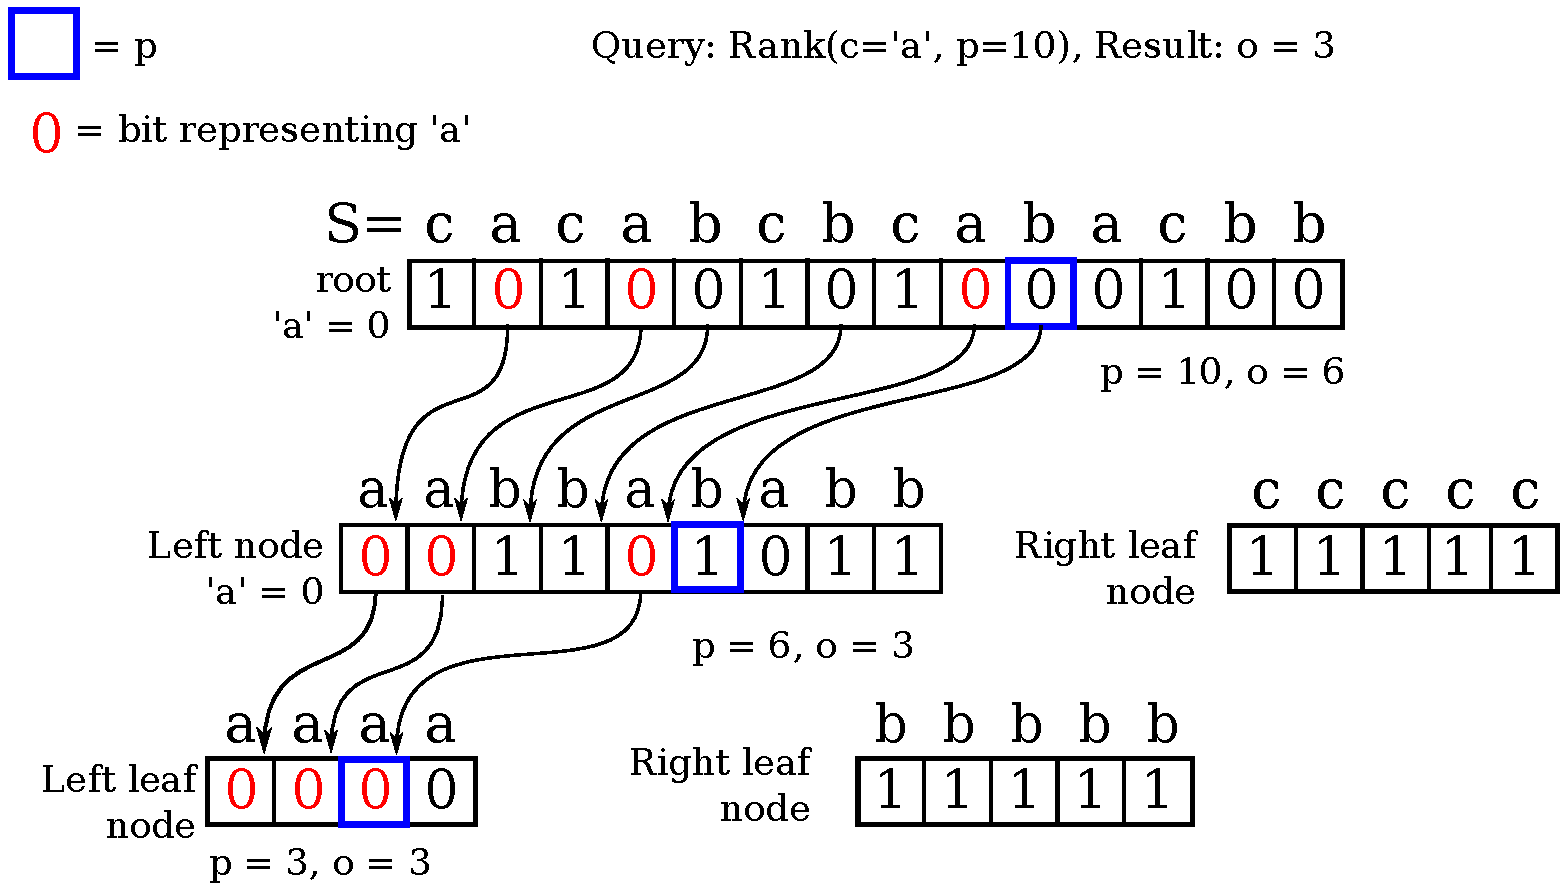
\includegraphics[width=0.8\textwidth]{RankDrawing}
\end{center}
\end{frame}

%------------------------------------------------

\subsection{Select}
\begin{frame}
\frametitle{Select on a Wavelet Tree}
\begin{center}
	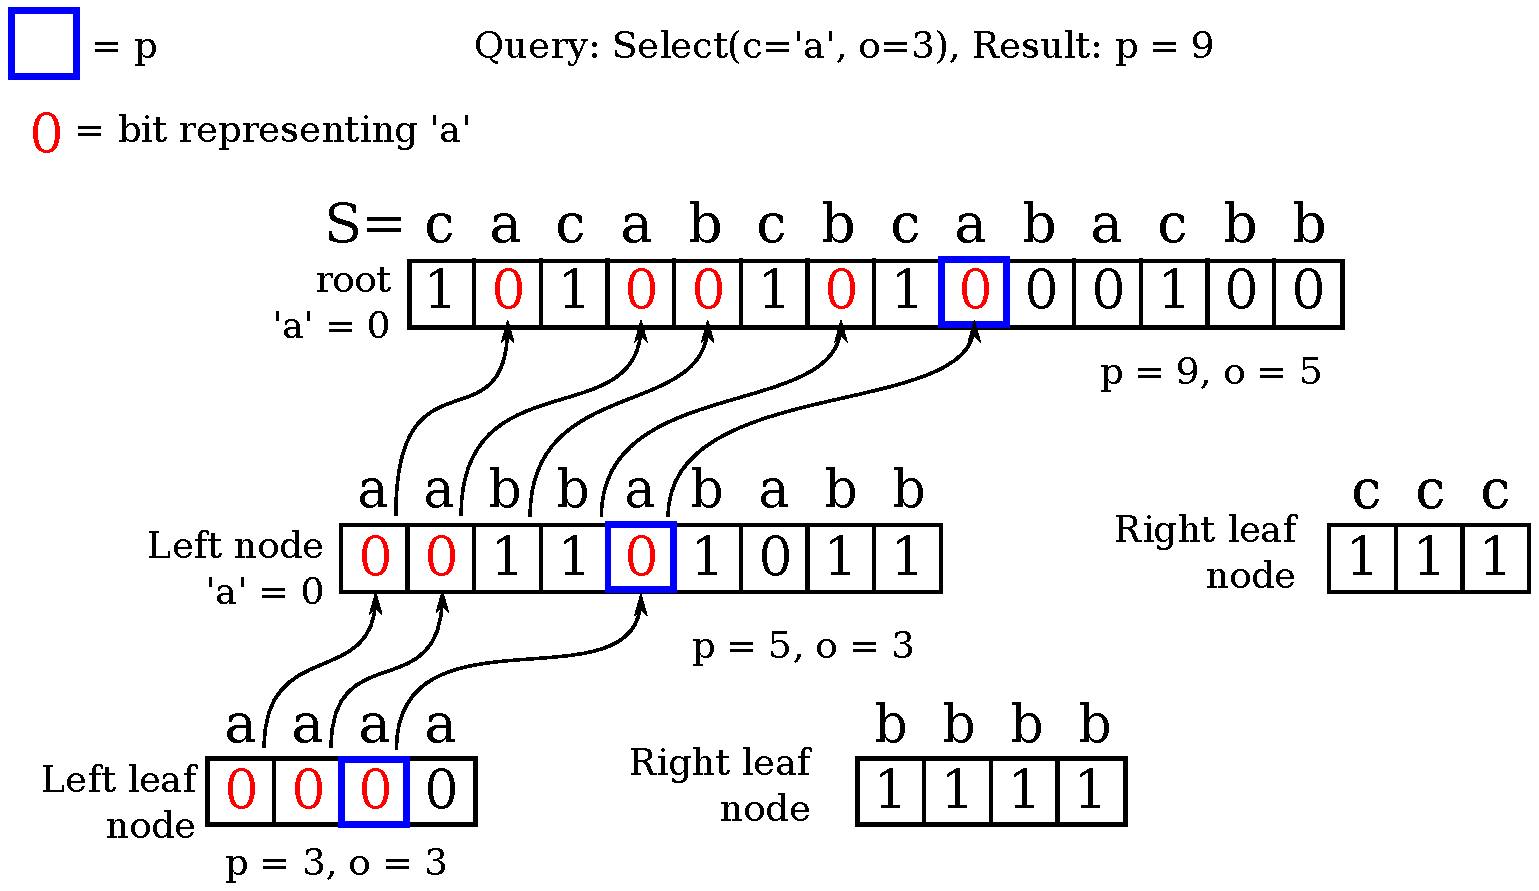
\includegraphics[width=0.8\textwidth]{SelectDrawing}
\end{center}
\end{frame}

\section{Applications}
%------------------------------------------------
\begin{frame}
\frametitle{Wavelet Tree: Applications}
\begin{center} \Huge{Applications} \end{center}
\end{frame}
%------------------------------------------------

\subsection{Information Retrieval}
\begin{frame}
\frametitle{Information Retrieval: Applications}
\begin{itemize}
\item Information Retrieval
	\begin{itemize}
	\item Positional inverted index
	\item Document retrieval
	\item Range Quantile Query: Return the \textit{k}th smallest number within a subsequence of a given sequence of elements.
	\item FM-count: Return number of occurrences of a pattern p in S. 
	\end{itemize}
\end{itemize}
\end{frame}

%------------------------------------------------
\subsection{Compression}
\begin{frame}
\frametitle{Compression: Applications}
\begin{itemize}
\item Compression
	\begin{itemize}
	\item Zero-order entropy compression ($H_0$) using a RLE Wavelet Tree or a Huffman Shaped Wavelet Tree.
	\item Higher-order entropy compression ($H_k$) using Burrows-Wheeler transformation and a RLE wavelet tree.
	\item $H_k <= H_0 <= \log \sigma$.
	\end{itemize}
\end{itemize}
\end{frame}

\subsubsection{Run-length encoding}
\begin{frame}
\frametitle{Compression: Run-length encoding}
\begin{itemize}
\item Run-length encoding counts the number of consecutive occurrences of a symbol and substitutes the consecutive occurrences with the symbol followed by its number of occurrences.
\item Example: $RLE(\text{aaaaabbbaacccccaaaaa}) = \text{a5,b3,a2,c5,a5}$.
\item Binary example: $RLE(00000000001111100000) = 10,5,5 $
	\begin{itemize}
	\item We can avoid specifying the symbol by assuming that $0$ is always the first symbol.
	\item If the binary number begins with a $1$ we just add a $0$ to the beginning of the result.
	\end{itemize}
\item Query by reversing RLE. It takes linear time $O(n)$ to reverse. Rank and select query time becomes $O(2n \log \sigma) = O(n \log \sigma)$
\item Achieves space complexity within $H_0$
\end{itemize}
\end{frame}


%------------------------------------------------
\begin{frame}
\frametitle{RLE Wavelet Tree on string \textit{bananahat} with alphabet $\Sigma =$ \textit{abhnt}}
\begin{figure}
\begin{subfigure}{0.49\textwidth}     
\Tree
%root
[.bananahat\\001010001 !\qsetw{3cm} 
	%left child
	[.baaaha\\000011 !\qsetw{3cm}
		[.baaaa\\10000 !\qsetw{3cm}
			[.aaaa !\qsetw{3cm} ]
			[.b !\qsetw{3cm} ]		
		] 
		[.h !\qsetw{3cm} ]
	] 
	%right child
	[.nnt\\001 !\qsetw{3cm}	
		[.nn !\qsetw{3cm} ] 
		[.t !\qsetw{3cm} ]
	]
]
		\caption{Wavelet Tree on string \textit{bananahat} with alphabet $\Sigma =$ \textit{abhnt}}
\end{subfigure}
\hfill
\begin{subfigure}{0.49\textwidth}	
\Tree
%root
[.bananahat\\2,1,1,1,3,1 !\qsetw{3cm} 
	%left child
	[.baaaha\\4,1,1 !\qsetw{3cm}
		[.baaaa\\0,1,4 !\qsetw{3cm}
			[.aaaa !\qsetw{3cm} ]
			[.b !\qsetw{3cm} ]		
		] 
		[.h !\qsetw{3cm} ]
	] 
	%right child
	[.nnt\\2,1 !\qsetw{3cm}	
		[.nn !\qsetw{3cm} ] 
		[.t !\qsetw{3cm} ]
	]
]
\caption{RLE Wavelet Tree on string \textit{bananahat} with alphabet $\Sigma =$ \textit{abhnt}}
\end{subfigure}
\end{figure}
\end{frame}


\subsubsection{Burrows-Wheeler Transform}
%------------------------------------------------
\begin{frame}
\frametitle{Compression: Burrows-Wheeler transform}
\begin{itemize}
\item BWT permutes the order of the characters. If the original string had several substrings that occurred often, then the transformed string will have several places where a single character is repeated multiple times in a row.
\item As a result it groups symbols more which improves the effect of Run-length encoding
\item BWT is reversible
\item Combined with RLE Wavelet Tree it achieves $H_k$ compression.
\end{itemize}
\end{frame}

\begin{frame}
\frametitle{BWT example}
$S = $ bananahat.
\begin{center}
$\begin{bmatrix}
	bananahat\#\\
	ananahat\#b\\
	nanahat\#ba\\
	anahat\#ban\\
	nahat\#bana\\
	ahat\#banan\\
	hat\#banana\\
	at\#bananah\\
	t\#bananaha\\
	\#bananahat\\
\end{bmatrix} \Rightarrow
\begin{bmatrix}
	\#bananaha\textbf{t}\\
	ahat\#bana\textbf{n}\\
	anahat\#ba\textbf{n}\\
	ananahat\#\textbf{b}\\
	at\#banana\textbf{h}\\
	bananahat\#\\
	hat\#banan\textbf{a}\\
	nahat\#ban\textbf{a}\\
	nanahat\#b\textbf{a}\\
	t\#bananah\textbf{a}
\end{bmatrix}$
\end{center}
$BWT(S) = $ tnnbhaaaa.
\end{frame}

%------------------------------------------------
\begin{frame}
\frametitle{Burrows-Wheeler reverse transform example}
$S = \text{dca}$
\begin{center}
$M = \begin{bmatrix}
	dca\#\\
	ca\#d\\
	a\#dc\\
	\#dca
\end{bmatrix} \Rightarrow
M' = 
\begin{bmatrix}
	\#dc\textbf{a}\\
	a\#d\textbf{c}\\
	ca\#\textbf{d}\\
	dca\textbf{\#}
\end{bmatrix}$\\
\end{center}
$BWT(S) = acd$
\vspace{0.5cm}

Reverse BWT:
\begin{tabular}{|l|l|l|l|l|l|l|l|}
\hline
Add 1 & Sort 1 & Add 2 & Sort 2 & Add 3 & Sort 3 & Add 4 & Sort 4\\
\hline 
\begin{tabular}{@{}>{$}l<{$}@{}}
	a\\ c\\ d\\ \#
\end{tabular} & 
\begin{tabular}{@{}>{$}l<{$}@{}}
	\#\\ a\\ c\\ d
\end{tabular} & 
\begin{tabular}{@{}>{$}l<{$}@{}}
	a\#\\ ca\\ dc\\ \#d
\end{tabular} & 
\begin{tabular}{@{}>{$}l<{$}@{}}
	\#d\\ a\#\\ ca\\ dc
\end{tabular} & 
\begin{tabular}{@{}>{$}l<{$}@{}}
	a\#d\\ ca\#\\ dca\\ \#dc
\end{tabular} & 
\begin{tabular}{@{}>{$}l<{$}@{}}
	\#dc\\ a\#d\\ ca\#\\ dca
\end{tabular} & 
\begin{tabular}{@{}>{$}l<{$}@{}}
	a\#dc\\ ca\#d\\ dca\#\\ \#dca
\end{tabular} &
\begin{tabular}{@{}>{$}l<{$}@{}}
	\#dca\\ a\#dc\\ ca\#d\\ \textbf{dca\#}\\
\end{tabular} \\ \hline
\end{tabular}
*$\# = \text{end of line character}$
\end{frame}

%----------------------------------------------------------------------------------------
\begin{frame}
\frametitle{RLE Wavelet Tree on string \textit{bananahat} with alphabet $\Sigma =$ \textit{abhnt}}
\begin{figure}
\begin{subfigure}{0.49\textwidth}     
\Tree
%root
[.bananahat\\2,1,1,1,3,1 !\qsetw{3cm} 
	%left child
	[.baaaha\\4,1,1 !\qsetw{3cm}
		[.baaaa\\0,1,4 !\qsetw{3cm}
			[.aaaa !\qsetw{3cm} ]
			[.b !\qsetw{3cm} ]		
		] 
		[.h !\qsetw{3cm} ]
	] 
	%right child
	[.nnt\\2,1 !\qsetw{3cm}	
		[.nn !\qsetw{3cm} ] 
		[.t !\qsetw{3cm} ]
	]
]
\caption{RLE Wavelet Tree on string \textit{bananahat} with alphabet $\Sigma =$ \textit{abhnt}}
\end{subfigure}
\hfill
\begin{subfigure}{0.49\textwidth}	
\Tree
%root
[.tnnbhaaaa\\\textbf{0,3,6} !\qsetw{3cm} 
	%left child
	[.bhaaaa\\1,1,4 !\qsetw{3cm} 
		[.baaaa\\0,1,4 !\qsetw{3cm} 
			[.aaaa !\qsetw{3cm} ]
			[.b !\qsetw{3cm} ]		
		] 
		[.h !\qsetw{3cm} ]
	] 
	%right child
	[.tnn\\0,1,2 !\qsetw{3cm}		
		[.nn !\qsetw{3cm} ] 
		[.t !\qsetw{3cm} ]
	]
]
\caption{BWT RLE Wavelet Tree on string \textit{tnnbhaaaa} with alphabet $\Sigma =$ \textit{abhnt}}
\end{subfigure}
\end{figure}
\end{frame}

\subsubsection{Huffman Shaped Wavelet tree}
%----------------------------------------------------------------------------------------
\begin{frame}
\frametitle{Huffman shaped wavelet tree}
\begin{itemize}
\item Use Huffman codes of symbols to shape the tree
\item A Huffman code is a binary value assigned to each symbol. The symbol with the highest frequency gets the lowest value.
\item Shaping the tree based on Huffman codes places the most frequent symbols at the top of the tree and least frequent symbols at the bottom of the tree.
\item Huffman shaping only makes sense on non-uniformly distributed data like a natural language text.

\end{itemize}
\end{frame}

%----------------------------------------------------------------------------------------
\begin{frame}
\frametitle{Huffman Shaped Wavelet Tree: Example}

\begin{figure}
\begin{subfigure}{0.49\textwidth}     
\Tree
%root
[.aaaaaabcaaaadf\\00000000000011 
	%left child
	[.aaaaaabcaaaa\\000000010000 
		[.aaaaaabaaaa\\00000010000 
			[.aaaaaaaaaa  ]
			[.b ]		
		] 
		[.c ]
	] 
	%right child
	[.df\\01 		
		[.d ] 
		[.f ]
	]
]
\caption{Balanced Wavelet tree: 39 bits}
\end{subfigure}
\hfill
\begin{subfigure}{0.49\textwidth}	
\Tree
%root
[.aaaaaabcaaaadf\\00000000000011 
	%left child
	[.bcdf\\0011  
		[.bc\\01  
			[.b  ]
			[.c  ]		
		] 
		[.df  
			[.d ]
			[.f ]
		]
	] 
	%right child
	[.aaaaaaaaaa\\01 ]
]
\caption{Huffman-shaped wavelet tree: 22 bits}
\end{subfigure}
\end{figure}

\end{frame}

%----------------------------------------------------------------------------------------
\begin{frame}
\frametitle{Huffman Shaped WT: Space complexity}
\begin{itemize}
\item Balanced version: $n \log \sigma + o(n \log\sigma) + O(\sigma \log n)$ bits
\item Huffman-shaped: $n(H_0(S) + 1) + o(n(H_0(S) + 1)) + O(\sigma \log n)$ bits. [Efficient Compressed Wavelet Trees over Large Alphabets by Navarro et al.]
\item Huffman-shaped + Compressed Bitmap (RLE): $nH_0(S) + o(n(H_0(S) + 1)) + O(\sigma \log n)$ bits.

\end{itemize}
\end{frame}

\section{Experiments and Results}
%----------------------------------------------------------------------------------------
\begin{frame}
\frametitle{Experiments and Results}
\huge{Experiments and Results}
\end{frame}

%----------------------------------------------------------------------------------------

\begin{frame}
\frametitle{Focus of experiments}
\begin{itemize}
\item Focus on optimizing and observing the effect of hardware penalties.
	\begin{itemize}
	\item Cache Misses.
	\item Branch Mispredictions.
	\item Translation Lookaside Buffer (TLB) Misses.
	\end{itemize}
\end{itemize}
\end{frame}

%----------------------------------------------------------------------------------------

\begin{frame}
\frametitle{Experiments}
\begin{itemize}
\item 1. Calculate binary rank and select using popcount
\item 2. Pre-compute binary rank values in blocks
\item 3. Block size dependence on input n
\item 4. Pre-compute cumulative sums of rank values
\item 5. Branchless select query
\item 6. Queries on skewed cumulative sum wavelet tree
\end{itemize}
\end{frame}

%----------------------------------------------------------------------------------------


\begin{frame}
\frametitle{Calculate binary rank and select using popcount}

\begin{figure}[h!]\tiny
	\begin{subfigure}{\textwidth}
		\center \scalebox{.6}{% GNUPLOT: LaTeX picture with Postscript
\begingroup
  \makeatletter
  \providecommand\color[2][]{%
    \GenericError{(gnuplot) \space\space\space\@spaces}{%
      Package color not loaded in conjunction with
      terminal option `colourtext'%
    }{See the gnuplot documentation for explanation.%
    }{Either use 'blacktext' in gnuplot or load the package
      color.sty in LaTeX.}%
    \renewcommand\color[2][]{}%
  }%
  \providecommand\includegraphics[2][]{%
    \GenericError{(gnuplot) \space\space\space\@spaces}{%
      Package graphicx or graphics not loaded%
    }{See the gnuplot documentation for explanation.%
    }{The gnuplot epslatex terminal needs graphicx.sty or graphics.sty.}%
    \renewcommand\includegraphics[2][]{}%
  }%
  \providecommand\rotatebox[2]{#2}%
  \@ifundefined{ifGPcolor}{%
    \newif\ifGPcolor
    \GPcolortrue
  }{}%
  \@ifundefined{ifGPblacktext}{%
    \newif\ifGPblacktext
    \GPblacktexttrue
  }{}%
  % define a \g@addto@macro without @ in the name:
  \let\gplgaddtomacro\g@addto@macro
  % define empty templates for all commands taking text:
  \gdef\gplbacktext{}%
  \gdef\gplfronttext{}%
  \makeatother
  \ifGPblacktext
    % no textcolor at all
    \def\colorrgb#1{}%
    \def\colorgray#1{}%
  \else
    % gray or color?
    \ifGPcolor
      \def\colorrgb#1{\color[rgb]{#1}}%
      \def\colorgray#1{\color[gray]{#1}}%
      \expandafter\def\csname LTw\endcsname{\color{white}}%
      \expandafter\def\csname LTb\endcsname{\color{black}}%
      \expandafter\def\csname LTa\endcsname{\color{black}}%
      \expandafter\def\csname LT0\endcsname{\color[rgb]{1,0,0}}%
      \expandafter\def\csname LT1\endcsname{\color[rgb]{0,1,0}}%
      \expandafter\def\csname LT2\endcsname{\color[rgb]{0,0,1}}%
      \expandafter\def\csname LT3\endcsname{\color[rgb]{1,0,1}}%
      \expandafter\def\csname LT4\endcsname{\color[rgb]{0,1,1}}%
      \expandafter\def\csname LT5\endcsname{\color[rgb]{1,1,0}}%
      \expandafter\def\csname LT6\endcsname{\color[rgb]{0,0,0}}%
      \expandafter\def\csname LT7\endcsname{\color[rgb]{1,0.3,0}}%
      \expandafter\def\csname LT8\endcsname{\color[rgb]{0.5,0.5,0.5}}%
    \else
      % gray
      \def\colorrgb#1{\color{black}}%
      \def\colorgray#1{\color[gray]{#1}}%
      \expandafter\def\csname LTw\endcsname{\color{white}}%
      \expandafter\def\csname LTb\endcsname{\color{black}}%
      \expandafter\def\csname LTa\endcsname{\color{black}}%
      \expandafter\def\csname LT0\endcsname{\color{black}}%
      \expandafter\def\csname LT1\endcsname{\color{black}}%
      \expandafter\def\csname LT2\endcsname{\color{black}}%
      \expandafter\def\csname LT3\endcsname{\color{black}}%
      \expandafter\def\csname LT4\endcsname{\color{black}}%
      \expandafter\def\csname LT5\endcsname{\color{black}}%
      \expandafter\def\csname LT6\endcsname{\color{black}}%
      \expandafter\def\csname LT7\endcsname{\color{black}}%
      \expandafter\def\csname LT8\endcsname{\color{black}}%
    \fi
  \fi
  \setlength{\unitlength}{0.0500bp}%
  \begin{picture}(7200.00,5040.00)%
    \gplgaddtomacro\gplbacktext{%
      \csname LTb\endcsname%
      \put(726,879){\makebox(0,0)[r]{\strut{} 0}}%
      \put(726,1269){\makebox(0,0)[r]{\strut{} 20}}%
      \put(726,1658){\makebox(0,0)[r]{\strut{} 40}}%
      \put(726,2048){\makebox(0,0)[r]{\strut{} 60}}%
      \put(726,2437){\makebox(0,0)[r]{\strut{} 80}}%
      \put(726,2827){\makebox(0,0)[r]{\strut{} 100}}%
      \put(726,3217){\makebox(0,0)[r]{\strut{} 120}}%
      \put(726,3606){\makebox(0,0)[r]{\strut{} 140}}%
      \put(726,3996){\makebox(0,0)[r]{\strut{} 160}}%
      \put(726,4385){\makebox(0,0)[r]{\strut{} 180}}%
      \put(726,4775){\makebox(0,0)[r]{\strut{} 200}}%
      \put(1263,747){\rotatebox{-30}{\makebox(0,0)[l]{\strut{}CPU Cycles}}}%
      \put(2074,747){\rotatebox{-30}{\makebox(0,0)[l]{\strut{}Wall Time}}}%
      \put(2885,747){\rotatebox{-30}{\makebox(0,0)[l]{\strut{}BM}}}%
      \put(3695,747){\rotatebox{-30}{\makebox(0,0)[l]{\strut{}TLBM}}}%
      \put(4506,747){\rotatebox{-30}{\makebox(0,0)[l]{\strut{}L1 CM}}}%
      \put(5317,747){\rotatebox{-30}{\makebox(0,0)[l]{\strut{}L2 CM}}}%
      \put(6127,747){\rotatebox{-30}{\makebox(0,0)[l]{\strut{}L3 CM}}}%
    }%
    \gplgaddtomacro\gplfronttext{%
      \csname LTb\endcsname%
      \put(5816,4602){\makebox(0,0)[r]{\strut{}Simple Binary Rank }}%
      \csname LTb\endcsname%
      \put(5816,4382){\makebox(0,0)[r]{\strut{}Binary Rank using Popcount}}%
    }%
    \gplbacktext
    \put(0,0){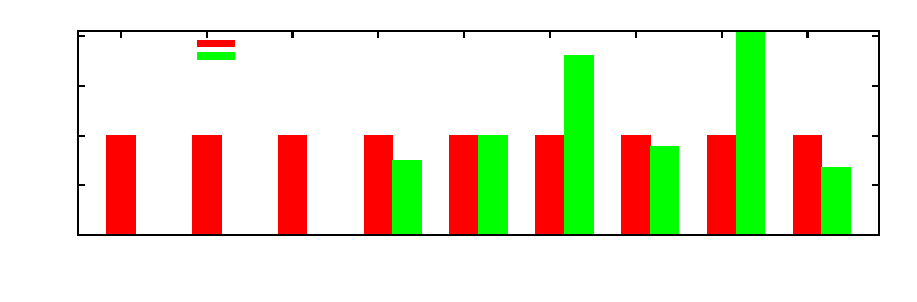
\includegraphics{popcountRankNew}}%
    \gplfronttext
  \end{picture}%
\endgroup
}
		\caption{\tiny{Rank}}
	\end{subfigure}
	\begin{subfigure}{\textwidth}
		\center \scalebox{.6}{% GNUPLOT: LaTeX picture with Postscript
\begingroup
  \makeatletter
  \providecommand\color[2][]{%
    \GenericError{(gnuplot) \space\space\space\@spaces}{%
      Package color not loaded in conjunction with
      terminal option `colourtext'%
    }{See the gnuplot documentation for explanation.%
    }{Either use 'blacktext' in gnuplot or load the package
      color.sty in LaTeX.}%
    \renewcommand\color[2][]{}%
  }%
  \providecommand\includegraphics[2][]{%
    \GenericError{(gnuplot) \space\space\space\@spaces}{%
      Package graphicx or graphics not loaded%
    }{See the gnuplot documentation for explanation.%
    }{The gnuplot epslatex terminal needs graphicx.sty or graphics.sty.}%
    \renewcommand\includegraphics[2][]{}%
  }%
  \providecommand\rotatebox[2]{#2}%
  \@ifundefined{ifGPcolor}{%
    \newif\ifGPcolor
    \GPcolortrue
  }{}%
  \@ifundefined{ifGPblacktext}{%
    \newif\ifGPblacktext
    \GPblacktexttrue
  }{}%
  % define a \g@addto@macro without @ in the name:
  \let\gplgaddtomacro\g@addto@macro
  % define empty templates for all commands taking text:
  \gdef\gplbacktext{}%
  \gdef\gplfronttext{}%
  \makeatother
  \ifGPblacktext
    % no textcolor at all
    \def\colorrgb#1{}%
    \def\colorgray#1{}%
  \else
    % gray or color?
    \ifGPcolor
      \def\colorrgb#1{\color[rgb]{#1}}%
      \def\colorgray#1{\color[gray]{#1}}%
      \expandafter\def\csname LTw\endcsname{\color{white}}%
      \expandafter\def\csname LTb\endcsname{\color{black}}%
      \expandafter\def\csname LTa\endcsname{\color{black}}%
      \expandafter\def\csname LT0\endcsname{\color[rgb]{1,0,0}}%
      \expandafter\def\csname LT1\endcsname{\color[rgb]{0,1,0}}%
      \expandafter\def\csname LT2\endcsname{\color[rgb]{0,0,1}}%
      \expandafter\def\csname LT3\endcsname{\color[rgb]{1,0,1}}%
      \expandafter\def\csname LT4\endcsname{\color[rgb]{0,1,1}}%
      \expandafter\def\csname LT5\endcsname{\color[rgb]{1,1,0}}%
      \expandafter\def\csname LT6\endcsname{\color[rgb]{0,0,0}}%
      \expandafter\def\csname LT7\endcsname{\color[rgb]{1,0.3,0}}%
      \expandafter\def\csname LT8\endcsname{\color[rgb]{0.5,0.5,0.5}}%
    \else
      % gray
      \def\colorrgb#1{\color{black}}%
      \def\colorgray#1{\color[gray]{#1}}%
      \expandafter\def\csname LTw\endcsname{\color{white}}%
      \expandafter\def\csname LTb\endcsname{\color{black}}%
      \expandafter\def\csname LTa\endcsname{\color{black}}%
      \expandafter\def\csname LT0\endcsname{\color{black}}%
      \expandafter\def\csname LT1\endcsname{\color{black}}%
      \expandafter\def\csname LT2\endcsname{\color{black}}%
      \expandafter\def\csname LT3\endcsname{\color{black}}%
      \expandafter\def\csname LT4\endcsname{\color{black}}%
      \expandafter\def\csname LT5\endcsname{\color{black}}%
      \expandafter\def\csname LT6\endcsname{\color{black}}%
      \expandafter\def\csname LT7\endcsname{\color{black}}%
      \expandafter\def\csname LT8\endcsname{\color{black}}%
    \fi
  \fi
  \setlength{\unitlength}{0.0500bp}%
  \begin{picture}(8496.00,2590.00)%
    \gplgaddtomacro\gplbacktext{%
      \csname LTb\endcsname%
      \put(516,479){\makebox(0,0)[r]{\strut{} 0}}%
      \put(516,959){\makebox(0,0)[r]{\strut{} 50}}%
      \put(516,1438){\makebox(0,0)[r]{\strut{} 100}}%
      \put(516,1918){\makebox(0,0)[r]{\strut{} 150}}%
      \put(516,2397){\makebox(0,0)[r]{\strut{} 200}}%
      \put(1000,407){\rotatebox{-30}{\makebox(0,0)[l]{\strut{}CPU Cycles}}}%
      \put(1824,407){\rotatebox{-30}{\makebox(0,0)[l]{\strut{}Wall Time}}}%
      \put(2648,407){\rotatebox{-30}{\makebox(0,0)[l]{\strut{}BM}}}%
      \put(3472,407){\rotatebox{-30}{\makebox(0,0)[l]{\strut{}TLBM}}}%
      \put(4296,407){\rotatebox{-30}{\makebox(0,0)[l]{\strut{}L1 CM}}}%
      \put(5120,407){\rotatebox{-30}{\makebox(0,0)[l]{\strut{}L2 CM}}}%
      \put(5944,407){\rotatebox{-30}{\makebox(0,0)[l]{\strut{}L2 CHits}}}%
      \put(6768,407){\rotatebox{-30}{\makebox(0,0)[l]{\strut{}L2 CM Rate}}}%
      \put(7592,407){\rotatebox{-30}{\makebox(0,0)[l]{\strut{}L3 CM}}}%
      \put(96,1462){\rotatebox{-270}{\makebox(0,0){\strut{}Percent of Simple}}}%
    }%
    \gplgaddtomacro\gplfronttext{%
      \csname LTb\endcsname%
      \put(1668,2322){\makebox(0,0)[r]{\strut{}Simple}}%
      \csname LTb\endcsname%
      \put(1668,2202){\makebox(0,0)[r]{\strut{}Using Popcount}}%
    }%
    \gplbacktext
    \put(0,0){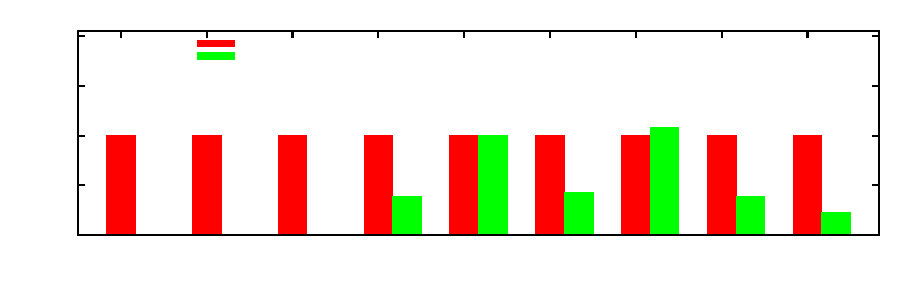
\includegraphics{popcountSelectNew}}%
    \gplfronttext
  \end{picture}%
\endgroup
}
		\caption{\tiny{Select}}
	\end{subfigure}
	\caption{\tiny{Rank and select queries using simple binary rank and select vs. rank and select queries using binary rank and select using the popcount instruction. Y-Axis is index 100 of the simple queries, that is, every value is percent of the value for the simple query.}}
\end{figure}
\end{frame}
%----------------------------------------------------------------------------------------
\begin{frame}
\frametitle{Experiments: Pre-compute binary rank values in blocks}
\begin{tabular}{|lcc|}
\hline
Name						& Concatenated Bitmaps	& Page-aligned Blocks	\\ \hline
Preallocated				& yes					& yes					\\ \hline
UnalignedPreallocated	& yes					& no						\\ \hline
Naive					& no						& yes					\\ \hline
UnalignedNaive			& no						& no						\\ \hline
\end{tabular}\\
\end{frame}
%----------------------------------------------------------------------------------------



\begin{frame}
\frametitle{Running time: Pre-compute binary rank values in blocks}
\begin{figure}
\begin{subfigure}{0.45\textwidth}
	\begin{tiny}	
	\scalebox{.7}{% GNUPLOT: LaTeX picture with Postscript
\begingroup
  \makeatletter
  \providecommand\color[2][]{%
    \GenericError{(gnuplot) \space\space\space\@spaces}{%
      Package color not loaded in conjunction with
      terminal option `colourtext'%
    }{See the gnuplot documentation for explanation.%
    }{Either use 'blacktext' in gnuplot or load the package
      color.sty in LaTeX.}%
    \renewcommand\color[2][]{}%
  }%
  \providecommand\includegraphics[2][]{%
    \GenericError{(gnuplot) \space\space\space\@spaces}{%
      Package graphicx or graphics not loaded%
    }{See the gnuplot documentation for explanation.%
    }{The gnuplot epslatex terminal needs graphicx.sty or graphics.sty.}%
    \renewcommand\includegraphics[2][]{}%
  }%
  \providecommand\rotatebox[2]{#2}%
  \@ifundefined{ifGPcolor}{%
    \newif\ifGPcolor
    \GPcolortrue
  }{}%
  \@ifundefined{ifGPblacktext}{%
    \newif\ifGPblacktext
    \GPblacktexttrue
  }{}%
  % define a \g@addto@macro without @ in the name:
  \let\gplgaddtomacro\g@addto@macro
  % define empty templates for all commands taking text:
  \gdef\gplbacktext{}%
  \gdef\gplfronttext{}%
  \makeatother
  \ifGPblacktext
    % no textcolor at all
    \def\colorrgb#1{}%
    \def\colorgray#1{}%
  \else
    % gray or color?
    \ifGPcolor
      \def\colorrgb#1{\color[rgb]{#1}}%
      \def\colorgray#1{\color[gray]{#1}}%
      \expandafter\def\csname LTw\endcsname{\color{white}}%
      \expandafter\def\csname LTb\endcsname{\color{black}}%
      \expandafter\def\csname LTa\endcsname{\color{black}}%
      \expandafter\def\csname LT0\endcsname{\color[rgb]{1,0,0}}%
      \expandafter\def\csname LT1\endcsname{\color[rgb]{0,1,0}}%
      \expandafter\def\csname LT2\endcsname{\color[rgb]{0,0,1}}%
      \expandafter\def\csname LT3\endcsname{\color[rgb]{1,0,1}}%
      \expandafter\def\csname LT4\endcsname{\color[rgb]{0,1,1}}%
      \expandafter\def\csname LT5\endcsname{\color[rgb]{1,1,0}}%
      \expandafter\def\csname LT6\endcsname{\color[rgb]{0,0,0}}%
      \expandafter\def\csname LT7\endcsname{\color[rgb]{1,0.3,0}}%
      \expandafter\def\csname LT8\endcsname{\color[rgb]{0.5,0.5,0.5}}%
    \else
      % gray
      \def\colorrgb#1{\color{black}}%
      \def\colorgray#1{\color[gray]{#1}}%
      \expandafter\def\csname LTw\endcsname{\color{white}}%
      \expandafter\def\csname LTb\endcsname{\color{black}}%
      \expandafter\def\csname LTa\endcsname{\color{black}}%
      \expandafter\def\csname LT0\endcsname{\color{black}}%
      \expandafter\def\csname LT1\endcsname{\color{black}}%
      \expandafter\def\csname LT2\endcsname{\color{black}}%
      \expandafter\def\csname LT3\endcsname{\color{black}}%
      \expandafter\def\csname LT4\endcsname{\color{black}}%
      \expandafter\def\csname LT5\endcsname{\color{black}}%
      \expandafter\def\csname LT6\endcsname{\color{black}}%
      \expandafter\def\csname LT7\endcsname{\color{black}}%
      \expandafter\def\csname LT8\endcsname{\color{black}}%
    \fi
  \fi
  \setlength{\unitlength}{0.0500bp}%
  \begin{picture}(7488.00,4464.00)%
    \gplgaddtomacro\gplbacktext{%
      \csname LTb\endcsname%
      \put(1210,704){\makebox(0,0)[r]{\strut{} 0}}%
      \put(1210,948){\makebox(0,0)[r]{\strut{} 2000}}%
      \put(1210,1193){\makebox(0,0)[r]{\strut{} 4000}}%
      \put(1210,1437){\makebox(0,0)[r]{\strut{} 6000}}%
      \put(1210,1682){\makebox(0,0)[r]{\strut{} 8000}}%
      \put(1210,1926){\makebox(0,0)[r]{\strut{} 10000}}%
      \put(1210,2170){\makebox(0,0)[r]{\strut{} 12000}}%
      \put(1210,2415){\makebox(0,0)[r]{\strut{} 14000}}%
      \put(1210,2659){\makebox(0,0)[r]{\strut{} 16000}}%
      \put(1342,484){\makebox(0,0){\strut{} 0}}%
      \put(1917,484){\makebox(0,0){\strut{} 20000}}%
      \put(2492,484){\makebox(0,0){\strut{} 40000}}%
      \put(3067,484){\makebox(0,0){\strut{} 60000}}%
      \put(3642,484){\makebox(0,0){\strut{} 80000}}%
      \put(4217,484){\makebox(0,0){\strut{} 100000}}%
      \put(4791,484){\makebox(0,0){\strut{} 120000}}%
      \put(5366,484){\makebox(0,0){\strut{} 140000}}%
      \put(5941,484){\makebox(0,0){\strut{} 160000}}%
      \put(6516,484){\makebox(0,0){\strut{} 180000}}%
      \put(7091,484){\makebox(0,0){\strut{} 200000}}%
      \put(176,1681){\rotatebox{-270}{\makebox(0,0){\strut{}Wall Time}}}%
      \put(4216,154){\makebox(0,0){\strut{}Block Size in bits}}%
    }%
    \gplgaddtomacro\gplfronttext{%
      \csname LTb\endcsname%
      \put(6600,4181){\makebox(0,0)[r]{\strut{}NaivePrecomputed, $mr\hat{\sigma}= $0.63 $avg\hat{\sigma}= $1.297}}%
      \csname LTb\endcsname%
      \put(6600,3741){\makebox(0,0)[r]{\strut{}PreallocatedPrecomputed, $mr\hat{\sigma}= $3.33 $avg\hat{\sigma}= $11.794}}%
      \csname LTb\endcsname%
      \put(6600,3301){\makebox(0,0)[r]{\strut{}UnalignedNaivePrecomputed, $mr\hat{\sigma}= $0.69 $avg\hat{\sigma}= $1.875}}%
    }%
    \gplbacktext
    \put(0,0){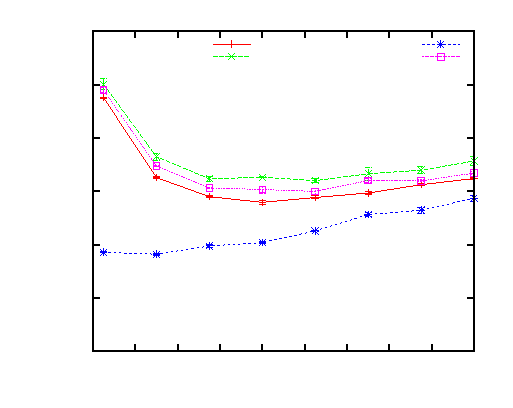
\includegraphics{PrecomputedRankBlockSize_Rank_WallTime}}%
    \gplfronttext
  \end{picture}%
\endgroup
}
	\end{tiny}
	\caption{Rank: Running Time}
\end{subfigure}
\hfill
\begin{subfigure}{0.45\textwidth}
	\begin{tiny}	
	\scalebox{.7}{% GNUPLOT: LaTeX picture with Postscript
\begingroup
  \makeatletter
  \providecommand\color[2][]{%
    \GenericError{(gnuplot) \space\space\space\@spaces}{%
      Package color not loaded in conjunction with
      terminal option `colourtext'%
    }{See the gnuplot documentation for explanation.%
    }{Either use 'blacktext' in gnuplot or load the package
      color.sty in LaTeX.}%
    \renewcommand\color[2][]{}%
  }%
  \providecommand\includegraphics[2][]{%
    \GenericError{(gnuplot) \space\space\space\@spaces}{%
      Package graphicx or graphics not loaded%
    }{See the gnuplot documentation for explanation.%
    }{The gnuplot epslatex terminal needs graphicx.sty or graphics.sty.}%
    \renewcommand\includegraphics[2][]{}%
  }%
  \providecommand\rotatebox[2]{#2}%
  \@ifundefined{ifGPcolor}{%
    \newif\ifGPcolor
    \GPcolortrue
  }{}%
  \@ifundefined{ifGPblacktext}{%
    \newif\ifGPblacktext
    \GPblacktexttrue
  }{}%
  % define a \g@addto@macro without @ in the name:
  \let\gplgaddtomacro\g@addto@macro
  % define empty templates for all commands taking text:
  \gdef\gplbacktext{}%
  \gdef\gplfronttext{}%
  \makeatother
  \ifGPblacktext
    % no textcolor at all
    \def\colorrgb#1{}%
    \def\colorgray#1{}%
  \else
    % gray or color?
    \ifGPcolor
      \def\colorrgb#1{\color[rgb]{#1}}%
      \def\colorgray#1{\color[gray]{#1}}%
      \expandafter\def\csname LTw\endcsname{\color{white}}%
      \expandafter\def\csname LTb\endcsname{\color{black}}%
      \expandafter\def\csname LTa\endcsname{\color{black}}%
      \expandafter\def\csname LT0\endcsname{\color[rgb]{1,0,0}}%
      \expandafter\def\csname LT1\endcsname{\color[rgb]{0,1,0}}%
      \expandafter\def\csname LT2\endcsname{\color[rgb]{0,0,1}}%
      \expandafter\def\csname LT3\endcsname{\color[rgb]{1,0,1}}%
      \expandafter\def\csname LT4\endcsname{\color[rgb]{0,1,1}}%
      \expandafter\def\csname LT5\endcsname{\color[rgb]{1,1,0}}%
      \expandafter\def\csname LT6\endcsname{\color[rgb]{0,0,0}}%
      \expandafter\def\csname LT7\endcsname{\color[rgb]{1,0.3,0}}%
      \expandafter\def\csname LT8\endcsname{\color[rgb]{0.5,0.5,0.5}}%
    \else
      % gray
      \def\colorrgb#1{\color{black}}%
      \def\colorgray#1{\color[gray]{#1}}%
      \expandafter\def\csname LTw\endcsname{\color{white}}%
      \expandafter\def\csname LTb\endcsname{\color{black}}%
      \expandafter\def\csname LTa\endcsname{\color{black}}%
      \expandafter\def\csname LT0\endcsname{\color{black}}%
      \expandafter\def\csname LT1\endcsname{\color{black}}%
      \expandafter\def\csname LT2\endcsname{\color{black}}%
      \expandafter\def\csname LT3\endcsname{\color{black}}%
      \expandafter\def\csname LT4\endcsname{\color{black}}%
      \expandafter\def\csname LT5\endcsname{\color{black}}%
      \expandafter\def\csname LT6\endcsname{\color{black}}%
      \expandafter\def\csname LT7\endcsname{\color{black}}%
      \expandafter\def\csname LT8\endcsname{\color{black}}%
    \fi
  \fi
  \setlength{\unitlength}{0.0500bp}%
  \begin{picture}(7488.00,4464.00)%
    \gplgaddtomacro\gplbacktext{%
      \csname LTb\endcsname%
      \put(1210,704){\makebox(0,0)[r]{\strut{} 0}}%
      \put(1210,1227){\makebox(0,0)[r]{\strut{} 5000}}%
      \put(1210,1750){\makebox(0,0)[r]{\strut{} 10000}}%
      \put(1210,2273){\makebox(0,0)[r]{\strut{} 15000}}%
      \put(1210,2796){\makebox(0,0)[r]{\strut{} 20000}}%
      \put(1210,3319){\makebox(0,0)[r]{\strut{} 25000}}%
      \put(1342,484){\makebox(0,0){\strut{} 0}}%
      \put(2300,484){\makebox(0,0){\strut{} 0.5}}%
      \put(3258,484){\makebox(0,0){\strut{} 1}}%
      \put(4217,484){\makebox(0,0){\strut{} 1.5}}%
      \put(5175,484){\makebox(0,0){\strut{} 2}}%
      \put(6133,484){\makebox(0,0){\strut{} 2.5}}%
      \put(7091,484){\makebox(0,0){\strut{} 3}}%
      \put(176,2011){\rotatebox{-270}{\makebox(0,0){\strut{}Wall Time ($\mu s$)}}}%
      \put(4216,154){\makebox(0,0){\strut{}Block Size (number of pages)}}%
    }%
    \gplgaddtomacro\gplfronttext{%
      \csname LTb\endcsname%
      \put(6468,4291){\makebox(0,0)[r]{\strut{}NaivePrecomputed, $mr\hat{\sigma}=$ 1.76 $avg\hat{\sigma}=$ 0.81}}%
      \csname LTb\endcsname%
      \put(6468,4071){\makebox(0,0)[r]{\strut{}PreallocatedPrecomputed, $mr\hat{\sigma}=$ 1.13 $avg\hat{\sigma}=$ 0.41}}%
      \csname LTb\endcsname%
      \put(6468,3851){\makebox(0,0)[r]{\strut{}UnalignedNaivePrecomputed, $mr\hat{\sigma}=$ 2.07 $avg\hat{\sigma}=$ 0.66}}%
    }%
    \gplbacktext
    \put(0,0){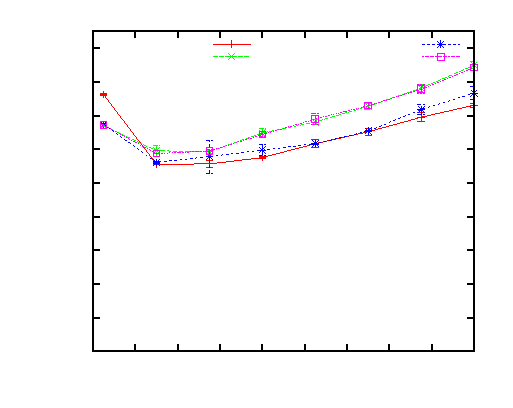
\includegraphics{PrecomputedRankBlockSize_Select_WallTime}}%
    \gplfronttext
  \end{picture}%
\endgroup
}
	\end{tiny}
	\caption{Select: Running Time}
\end{subfigure}
\end{figure}
Best Block size: $\frac{1}{2}$ page size = $\frac{1}{2}*4096 \text{ bytes} = 2048 \text{ bytes}$.
\end{frame}


\begin{frame}
\frametitle{Memory usage: Pre-compute binary rank values in blocks}
\begin{center}
\begin{tiny}
% GNUPLOT: LaTeX picture with Postscript
\begingroup
  \makeatletter
  \providecommand\color[2][]{%
    \GenericError{(gnuplot) \space\space\space\@spaces}{%
      Package color not loaded in conjunction with
      terminal option `colourtext'%
    }{See the gnuplot documentation for explanation.%
    }{Either use 'blacktext' in gnuplot or load the package
      color.sty in LaTeX.}%
    \renewcommand\color[2][]{}%
  }%
  \providecommand\includegraphics[2][]{%
    \GenericError{(gnuplot) \space\space\space\@spaces}{%
      Package graphicx or graphics not loaded%
    }{See the gnuplot documentation for explanation.%
    }{The gnuplot epslatex terminal needs graphicx.sty or graphics.sty.}%
    \renewcommand\includegraphics[2][]{}%
  }%
  \providecommand\rotatebox[2]{#2}%
  \@ifundefined{ifGPcolor}{%
    \newif\ifGPcolor
    \GPcolortrue
  }{}%
  \@ifundefined{ifGPblacktext}{%
    \newif\ifGPblacktext
    \GPblacktexttrue
  }{}%
  % define a \g@addto@macro without @ in the name:
  \let\gplgaddtomacro\g@addto@macro
  % define empty templates for all commands taking text:
  \gdef\gplbacktext{}%
  \gdef\gplfronttext{}%
  \makeatother
  \ifGPblacktext
    % no textcolor at all
    \def\colorrgb#1{}%
    \def\colorgray#1{}%
  \else
    % gray or color?
    \ifGPcolor
      \def\colorrgb#1{\color[rgb]{#1}}%
      \def\colorgray#1{\color[gray]{#1}}%
      \expandafter\def\csname LTw\endcsname{\color{white}}%
      \expandafter\def\csname LTb\endcsname{\color{black}}%
      \expandafter\def\csname LTa\endcsname{\color{black}}%
      \expandafter\def\csname LT0\endcsname{\color[rgb]{1,0,0}}%
      \expandafter\def\csname LT1\endcsname{\color[rgb]{0,1,0}}%
      \expandafter\def\csname LT2\endcsname{\color[rgb]{0,0,1}}%
      \expandafter\def\csname LT3\endcsname{\color[rgb]{1,0,1}}%
      \expandafter\def\csname LT4\endcsname{\color[rgb]{0,1,1}}%
      \expandafter\def\csname LT5\endcsname{\color[rgb]{1,1,0}}%
      \expandafter\def\csname LT6\endcsname{\color[rgb]{0,0,0}}%
      \expandafter\def\csname LT7\endcsname{\color[rgb]{1,0.3,0}}%
      \expandafter\def\csname LT8\endcsname{\color[rgb]{0.5,0.5,0.5}}%
    \else
      % gray
      \def\colorrgb#1{\color{black}}%
      \def\colorgray#1{\color[gray]{#1}}%
      \expandafter\def\csname LTw\endcsname{\color{white}}%
      \expandafter\def\csname LTb\endcsname{\color{black}}%
      \expandafter\def\csname LTa\endcsname{\color{black}}%
      \expandafter\def\csname LT0\endcsname{\color{black}}%
      \expandafter\def\csname LT1\endcsname{\color{black}}%
      \expandafter\def\csname LT2\endcsname{\color{black}}%
      \expandafter\def\csname LT3\endcsname{\color{black}}%
      \expandafter\def\csname LT4\endcsname{\color{black}}%
      \expandafter\def\csname LT5\endcsname{\color{black}}%
      \expandafter\def\csname LT6\endcsname{\color{black}}%
      \expandafter\def\csname LT7\endcsname{\color{black}}%
      \expandafter\def\csname LT8\endcsname{\color{black}}%
    \fi
  \fi
  \setlength{\unitlength}{0.0500bp}%
  \begin{picture}(7488.00,4464.00)%
    \gplgaddtomacro\gplbacktext{%
      \csname LTb\endcsname%
      \put(1342,704){\makebox(0,0)[r]{\strut{} 820000}}%
      \put(1342,948){\makebox(0,0)[r]{\strut{} 830000}}%
      \put(1342,1193){\makebox(0,0)[r]{\strut{} 840000}}%
      \put(1342,1437){\makebox(0,0)[r]{\strut{} 850000}}%
      \put(1342,1682){\makebox(0,0)[r]{\strut{} 860000}}%
      \put(1342,1926){\makebox(0,0)[r]{\strut{} 870000}}%
      \put(1342,2170){\makebox(0,0)[r]{\strut{} 880000}}%
      \put(1342,2415){\makebox(0,0)[r]{\strut{} 890000}}%
      \put(1342,2659){\makebox(0,0)[r]{\strut{} 900000}}%
      \put(1474,484){\makebox(0,0){\strut{} 0}}%
      \put(2036,484){\makebox(0,0){\strut{} 20}}%
      \put(2597,484){\makebox(0,0){\strut{} 40}}%
      \put(3159,484){\makebox(0,0){\strut{} 60}}%
      \put(3721,484){\makebox(0,0){\strut{} 80}}%
      \put(4283,484){\makebox(0,0){\strut{} 100}}%
      \put(4844,484){\makebox(0,0){\strut{} 120}}%
      \put(5406,484){\makebox(0,0){\strut{} 140}}%
      \put(5968,484){\makebox(0,0){\strut{} 160}}%
      \put(6529,484){\makebox(0,0){\strut{} 180}}%
      \put(7091,484){\makebox(0,0){\strut{} 200}}%
      \put(176,1681){\rotatebox{-270}{\makebox(0,0){\strut{}Memory Usage}}}%
      \put(4282,154){\makebox(0,0){\strut{}Block Size  (x1000 bits)}}%
    }%
    \gplgaddtomacro\gplfronttext{%
      \csname LTb\endcsname%
      \put(6236,4181){\makebox(0,0)[r]{\strut{}NaivePrecomputed, $mr\hat{\sigma}=$1.30 $avg\hat{\sigma}=$0.63}}%
      \csname LTb\endcsname%
      \put(6236,3741){\makebox(0,0)[r]{\strut{}PreallocatedPrecomputed, $mr\hat{\sigma}=$11.79 $avg\hat{\sigma}=$3.33}}%
      \csname LTb\endcsname%
      \put(6236,3301){\makebox(0,0)[r]{\strut{}UnalignedNaivePrecomputed, $mr\hat{\sigma}=$1.88 $avg\hat{\sigma}=$0.69}}%
    }%
    \gplbacktext
    \put(0,0){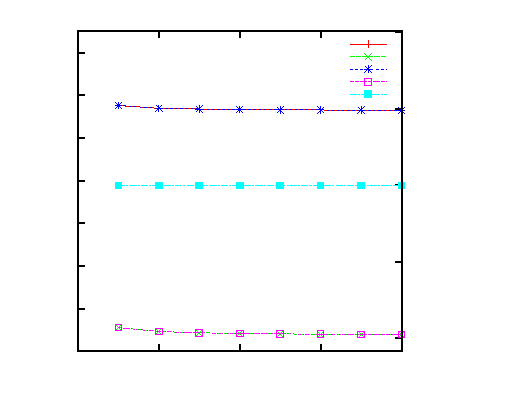
\includegraphics{PrecomputedRankBlockSize_MemoryUsage}}%
    \gplfronttext
  \end{picture}%
\endgroup

\end{tiny}
\end{center}
\end{frame}

\begin{frame}
\frametitle{Running time: Not precomputed vs. best precomputed}
\begin{figure}
	\begin{subfigure}{0.48\textwidth}
		\begin{tiny}
		\scalebox{.7}{% GNUPLOT: LaTeX picture with Postscript
\begingroup
  \makeatletter
  \providecommand\color[2][]{%
    \GenericError{(gnuplot) \space\space\space\@spaces}{%
      Package color not loaded in conjunction with
      terminal option `colourtext'%
    }{See the gnuplot documentation for explanation.%
    }{Either use 'blacktext' in gnuplot or load the package
      color.sty in LaTeX.}%
    \renewcommand\color[2][]{}%
  }%
  \providecommand\includegraphics[2][]{%
    \GenericError{(gnuplot) \space\space\space\@spaces}{%
      Package graphicx or graphics not loaded%
    }{See the gnuplot documentation for explanation.%
    }{The gnuplot epslatex terminal needs graphicx.sty or graphics.sty.}%
    \renewcommand\includegraphics[2][]{}%
  }%
  \providecommand\rotatebox[2]{#2}%
  \@ifundefined{ifGPcolor}{%
    \newif\ifGPcolor
    \GPcolortrue
  }{}%
  \@ifundefined{ifGPblacktext}{%
    \newif\ifGPblacktext
    \GPblacktexttrue
  }{}%
  % define a \g@addto@macro without @ in the name:
  \let\gplgaddtomacro\g@addto@macro
  % define empty templates for all commands taking text:
  \gdef\gplbacktext{}%
  \gdef\gplfronttext{}%
  \makeatother
  \ifGPblacktext
    % no textcolor at all
    \def\colorrgb#1{}%
    \def\colorgray#1{}%
  \else
    % gray or color?
    \ifGPcolor
      \def\colorrgb#1{\color[rgb]{#1}}%
      \def\colorgray#1{\color[gray]{#1}}%
      \expandafter\def\csname LTw\endcsname{\color{white}}%
      \expandafter\def\csname LTb\endcsname{\color{black}}%
      \expandafter\def\csname LTa\endcsname{\color{black}}%
      \expandafter\def\csname LT0\endcsname{\color[rgb]{1,0,0}}%
      \expandafter\def\csname LT1\endcsname{\color[rgb]{0,1,0}}%
      \expandafter\def\csname LT2\endcsname{\color[rgb]{0,0,1}}%
      \expandafter\def\csname LT3\endcsname{\color[rgb]{1,0,1}}%
      \expandafter\def\csname LT4\endcsname{\color[rgb]{0,1,1}}%
      \expandafter\def\csname LT5\endcsname{\color[rgb]{1,1,0}}%
      \expandafter\def\csname LT6\endcsname{\color[rgb]{0,0,0}}%
      \expandafter\def\csname LT7\endcsname{\color[rgb]{1,0.3,0}}%
      \expandafter\def\csname LT8\endcsname{\color[rgb]{0.5,0.5,0.5}}%
    \else
      % gray
      \def\colorrgb#1{\color{black}}%
      \def\colorgray#1{\color[gray]{#1}}%
      \expandafter\def\csname LTw\endcsname{\color{white}}%
      \expandafter\def\csname LTb\endcsname{\color{black}}%
      \expandafter\def\csname LTa\endcsname{\color{black}}%
      \expandafter\def\csname LT0\endcsname{\color{black}}%
      \expandafter\def\csname LT1\endcsname{\color{black}}%
      \expandafter\def\csname LT2\endcsname{\color{black}}%
      \expandafter\def\csname LT3\endcsname{\color{black}}%
      \expandafter\def\csname LT4\endcsname{\color{black}}%
      \expandafter\def\csname LT5\endcsname{\color{black}}%
      \expandafter\def\csname LT6\endcsname{\color{black}}%
      \expandafter\def\csname LT7\endcsname{\color{black}}%
      \expandafter\def\csname LT8\endcsname{\color{black}}%
    \fi
  \fi
  \setlength{\unitlength}{0.0500bp}%
  \begin{picture}(4608.00,3600.00)%
    \gplgaddtomacro\gplbacktext{%
      \csname LTb\endcsname%
      \put(516,144){\makebox(0,0)[r]{\strut{} 0}}%
      \put(516,558){\makebox(0,0)[r]{\strut{} 0.2}}%
      \put(516,972){\makebox(0,0)[r]{\strut{} 0.4}}%
      \put(516,1386){\makebox(0,0)[r]{\strut{} 0.6}}%
      \put(516,1800){\makebox(0,0)[r]{\strut{} 0.8}}%
      \put(516,2213){\makebox(0,0)[r]{\strut{} 1}}%
      \put(516,2627){\makebox(0,0)[r]{\strut{} 1.2}}%
      \put(516,3041){\makebox(0,0)[r]{\strut{} 1.4}}%
      \put(516,3455){\makebox(0,0)[r]{\strut{} 1.6}}%
      \put(96,1799){\rotatebox{-270}{\makebox(0,0){\strut{}Walltime (seconds)}}}%
    }%
    \gplgaddtomacro\gplfronttext{%
      \csname LTb\endcsname%
      \put(3824,3332){\makebox(0,0)[r]{\strut{}NaiveInteger}}%
      \csname LTb\endcsname%
      \put(3824,3212){\makebox(0,0)[r]{\strut{}UnalignedNaive}}%
    }%
    \gplbacktext
    \put(0,0){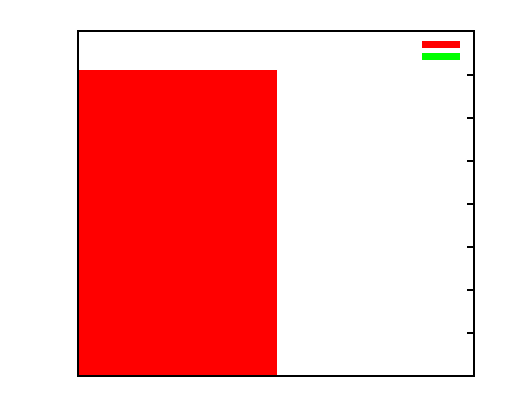
\includegraphics{PrecomputedRankBlockSize_vsNaiveInteger_Rank}}%
    \gplfronttext
  \end{picture}%
\endgroup
}
		\end{tiny}
		\caption{Rank}
	\end{subfigure}
	\hfill
	\begin{subfigure}{0.48\textwidth}
		\begin{tiny}
		\scalebox{.7}{% GNUPLOT: LaTeX picture with Postscript
\begingroup
  \makeatletter
  \providecommand\color[2][]{%
    \GenericError{(gnuplot) \space\space\space\@spaces}{%
      Package color not loaded in conjunction with
      terminal option `colourtext'%
    }{See the gnuplot documentation for explanation.%
    }{Either use 'blacktext' in gnuplot or load the package
      color.sty in LaTeX.}%
    \renewcommand\color[2][]{}%
  }%
  \providecommand\includegraphics[2][]{%
    \GenericError{(gnuplot) \space\space\space\@spaces}{%
      Package graphicx or graphics not loaded%
    }{See the gnuplot documentation for explanation.%
    }{The gnuplot epslatex terminal needs graphicx.sty or graphics.sty.}%
    \renewcommand\includegraphics[2][]{}%
  }%
  \providecommand\rotatebox[2]{#2}%
  \@ifundefined{ifGPcolor}{%
    \newif\ifGPcolor
    \GPcolortrue
  }{}%
  \@ifundefined{ifGPblacktext}{%
    \newif\ifGPblacktext
    \GPblacktexttrue
  }{}%
  % define a \g@addto@macro without @ in the name:
  \let\gplgaddtomacro\g@addto@macro
  % define empty templates for all commands taking text:
  \gdef\gplbacktext{}%
  \gdef\gplfronttext{}%
  \makeatother
  \ifGPblacktext
    % no textcolor at all
    \def\colorrgb#1{}%
    \def\colorgray#1{}%
  \else
    % gray or color?
    \ifGPcolor
      \def\colorrgb#1{\color[rgb]{#1}}%
      \def\colorgray#1{\color[gray]{#1}}%
      \expandafter\def\csname LTw\endcsname{\color{white}}%
      \expandafter\def\csname LTb\endcsname{\color{black}}%
      \expandafter\def\csname LTa\endcsname{\color{black}}%
      \expandafter\def\csname LT0\endcsname{\color[rgb]{1,0,0}}%
      \expandafter\def\csname LT1\endcsname{\color[rgb]{0,1,0}}%
      \expandafter\def\csname LT2\endcsname{\color[rgb]{0,0,1}}%
      \expandafter\def\csname LT3\endcsname{\color[rgb]{1,0,1}}%
      \expandafter\def\csname LT4\endcsname{\color[rgb]{0,1,1}}%
      \expandafter\def\csname LT5\endcsname{\color[rgb]{1,1,0}}%
      \expandafter\def\csname LT6\endcsname{\color[rgb]{0,0,0}}%
      \expandafter\def\csname LT7\endcsname{\color[rgb]{1,0.3,0}}%
      \expandafter\def\csname LT8\endcsname{\color[rgb]{0.5,0.5,0.5}}%
    \else
      % gray
      \def\colorrgb#1{\color{black}}%
      \def\colorgray#1{\color[gray]{#1}}%
      \expandafter\def\csname LTw\endcsname{\color{white}}%
      \expandafter\def\csname LTb\endcsname{\color{black}}%
      \expandafter\def\csname LTa\endcsname{\color{black}}%
      \expandafter\def\csname LT0\endcsname{\color{black}}%
      \expandafter\def\csname LT1\endcsname{\color{black}}%
      \expandafter\def\csname LT2\endcsname{\color{black}}%
      \expandafter\def\csname LT3\endcsname{\color{black}}%
      \expandafter\def\csname LT4\endcsname{\color{black}}%
      \expandafter\def\csname LT5\endcsname{\color{black}}%
      \expandafter\def\csname LT6\endcsname{\color{black}}%
      \expandafter\def\csname LT7\endcsname{\color{black}}%
      \expandafter\def\csname LT8\endcsname{\color{black}}%
    \fi
  \fi
  \setlength{\unitlength}{0.0500bp}%
  \begin{picture}(4608.00,3600.00)%
    \gplgaddtomacro\gplbacktext{%
      \csname LTb\endcsname%
      \put(516,144){\makebox(0,0)[r]{\strut{} 0}}%
      \put(516,512){\makebox(0,0)[r]{\strut{} 0.2}}%
      \put(516,880){\makebox(0,0)[r]{\strut{} 0.4}}%
      \put(516,1248){\makebox(0,0)[r]{\strut{} 0.6}}%
      \put(516,1616){\makebox(0,0)[r]{\strut{} 0.8}}%
      \put(516,1983){\makebox(0,0)[r]{\strut{} 1}}%
      \put(516,2351){\makebox(0,0)[r]{\strut{} 1.2}}%
      \put(516,2719){\makebox(0,0)[r]{\strut{} 1.4}}%
      \put(516,3087){\makebox(0,0)[r]{\strut{} 1.6}}%
      \put(516,3455){\makebox(0,0)[r]{\strut{} 1.8}}%
      \put(96,1799){\rotatebox{-270}{\makebox(0,0){\strut{}Walltime (seconds)}}}%
    }%
    \gplgaddtomacro\gplfronttext{%
      \csname LTb\endcsname%
      \put(3824,3332){\makebox(0,0)[r]{\strut{}NaiveInteger}}%
      \csname LTb\endcsname%
      \put(3824,3212){\makebox(0,0)[r]{\strut{}UnalignedNaive}}%
    }%
    \gplbacktext
    \put(0,0){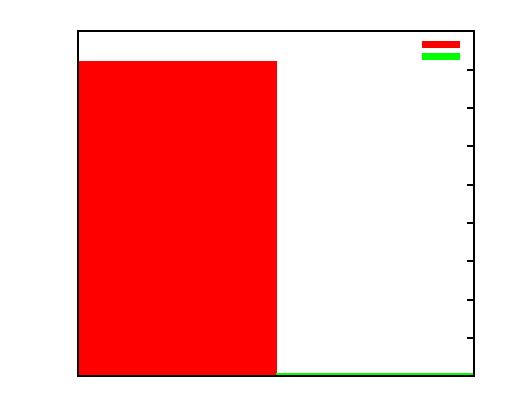
\includegraphics{PrecomputedRankBlockSize_vsNaiveInteger_Select}}%
    \gplfronttext
  \end{picture}%
\endgroup
}
		\end{tiny}
		\caption{Select}
	\end{subfigure}
	\caption{Comparison of wall time of rank and select queries between SimpleNaive not using precomputed values and UnalignedNaive using precomputed values.}
\end{figure}
\end{frame}

\begin{frame}
\frametitle{Block size dependence on input size n}
\begin{itemize}
\item When using lookups of precomputed values
It costs $O(\frac{n}{b} + b)$ to calculate the binary rank.
\item It costs $O(\frac{n}{b})$ to scan the blocks, and $O(b)$ to calculate the rank within a single block using popcount. The optimal block size should be one that minimizes this.
\item The derivative of $\frac{n}{b}+b$ is $1-\frac{n}{b^2}$ and its root is $n = b^2$ making the optimal block size $b = \sqrt{n}$.
\item This is only the optimal block size for a single bitmap, and a wavelet tree has many bitmaps of varying sizes $n$ that are lower near the leaves.
\end{itemize}
\end{frame}

\begin{frame}
\frametitle{Experiment: Block size dependence on input size n}
\begin{figure}\tiny
\begin{subfigure}{0.48\textwidth}
	\scalebox{.5}{% GNUPLOT: LaTeX picture with Postscript
\begingroup
  \makeatletter
  \providecommand\color[2][]{%
    \GenericError{(gnuplot) \space\space\space\@spaces}{%
      Package color not loaded in conjunction with
      terminal option `colourtext'%
    }{See the gnuplot documentation for explanation.%
    }{Either use 'blacktext' in gnuplot or load the package
      color.sty in LaTeX.}%
    \renewcommand\color[2][]{}%
  }%
  \providecommand\includegraphics[2][]{%
    \GenericError{(gnuplot) \space\space\space\@spaces}{%
      Package graphicx or graphics not loaded%
    }{See the gnuplot documentation for explanation.%
    }{The gnuplot epslatex terminal needs graphicx.sty or graphics.sty.}%
    \renewcommand\includegraphics[2][]{}%
  }%
  \providecommand\rotatebox[2]{#2}%
  \@ifundefined{ifGPcolor}{%
    \newif\ifGPcolor
    \GPcolortrue
  }{}%
  \@ifundefined{ifGPblacktext}{%
    \newif\ifGPblacktext
    \GPblacktexttrue
  }{}%
  % define a \g@addto@macro without @ in the name:
  \let\gplgaddtomacro\g@addto@macro
  % define empty templates for all commands taking text:
  \gdef\gplbacktext{}%
  \gdef\gplfronttext{}%
  \makeatother
  \ifGPblacktext
    % no textcolor at all
    \def\colorrgb#1{}%
    \def\colorgray#1{}%
  \else
    % gray or color?
    \ifGPcolor
      \def\colorrgb#1{\color[rgb]{#1}}%
      \def\colorgray#1{\color[gray]{#1}}%
      \expandafter\def\csname LTw\endcsname{\color{white}}%
      \expandafter\def\csname LTb\endcsname{\color{black}}%
      \expandafter\def\csname LTa\endcsname{\color{black}}%
      \expandafter\def\csname LT0\endcsname{\color[rgb]{1,0,0}}%
      \expandafter\def\csname LT1\endcsname{\color[rgb]{0,1,0}}%
      \expandafter\def\csname LT2\endcsname{\color[rgb]{0,0,1}}%
      \expandafter\def\csname LT3\endcsname{\color[rgb]{1,0,1}}%
      \expandafter\def\csname LT4\endcsname{\color[rgb]{0,1,1}}%
      \expandafter\def\csname LT5\endcsname{\color[rgb]{1,1,0}}%
      \expandafter\def\csname LT6\endcsname{\color[rgb]{0,0,0}}%
      \expandafter\def\csname LT7\endcsname{\color[rgb]{1,0.3,0}}%
      \expandafter\def\csname LT8\endcsname{\color[rgb]{0.5,0.5,0.5}}%
    \else
      % gray
      \def\colorrgb#1{\color{black}}%
      \def\colorgray#1{\color[gray]{#1}}%
      \expandafter\def\csname LTw\endcsname{\color{white}}%
      \expandafter\def\csname LTb\endcsname{\color{black}}%
      \expandafter\def\csname LTa\endcsname{\color{black}}%
      \expandafter\def\csname LT0\endcsname{\color{black}}%
      \expandafter\def\csname LT1\endcsname{\color{black}}%
      \expandafter\def\csname LT2\endcsname{\color{black}}%
      \expandafter\def\csname LT3\endcsname{\color{black}}%
      \expandafter\def\csname LT4\endcsname{\color{black}}%
      \expandafter\def\csname LT5\endcsname{\color{black}}%
      \expandafter\def\csname LT6\endcsname{\color{black}}%
      \expandafter\def\csname LT7\endcsname{\color{black}}%
      \expandafter\def\csname LT8\endcsname{\color{black}}%
    \fi
  \fi
  \setlength{\unitlength}{0.0500bp}%
  \begin{picture}(4608.00,3600.00)%
    \gplgaddtomacro\gplbacktext{%
      \csname LTb\endcsname%
      \put(588,384){\makebox(0,0)[r]{\strut{} 0}}%
      \put(588,998){\makebox(0,0)[r]{\strut{} 500}}%
      \put(588,1612){\makebox(0,0)[r]{\strut{} 1000}}%
      \put(588,2227){\makebox(0,0)[r]{\strut{} 1500}}%
      \put(588,2841){\makebox(0,0)[r]{\strut{} 2000}}%
      \put(588,3455){\makebox(0,0)[r]{\strut{} 2500}}%
      \put(660,264){\makebox(0,0){\strut{} 10}}%
      \put(1406,264){\makebox(0,0){\strut{} 100}}%
      \put(2152,264){\makebox(0,0){\strut{} 1000}}%
      \put(2899,264){\makebox(0,0){\strut{} 10000}}%
      \put(3645,264){\makebox(0,0){\strut{} 100000}}%
      \put(4391,264){\makebox(0,0){\strut{} 1e+06}}%
      \put(96,1919){\rotatebox{-270}{\makebox(0,0){\strut{}Wall Time ($\mu s$)}}}%
      \put(2525,84){\makebox(0,0){\strut{}Block Size (bits)}}%
    }%
    \gplgaddtomacro\gplfronttext{%
      \csname LTb\endcsname%
      \put(3824,3332){\makebox(0,0)[r]{\strut{}UnalignedNaive}}%
    }%
    \gplbacktext
    \put(0,0){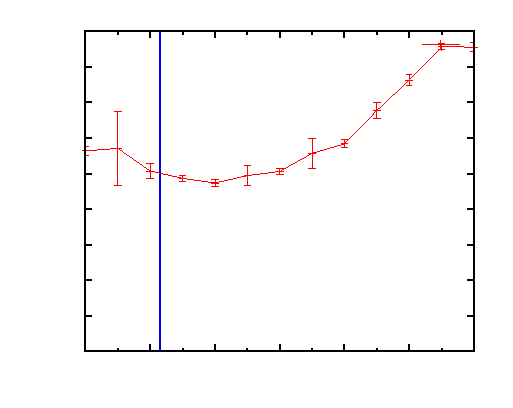
\includegraphics{PrecomputedRankBlockSizeVaryN_5_Rank_WallTime}}%
    \gplfronttext
  \end{picture}%
\endgroup
}
	\caption{$n = 10^5$}
\end{subfigure}
\hfill
\begin{subfigure}{0.48\textwidth}
	\scalebox{.5}{% GNUPLOT: LaTeX picture with Postscript
\begingroup
  \makeatletter
  \providecommand\color[2][]{%
    \GenericError{(gnuplot) \space\space\space\@spaces}{%
      Package color not loaded in conjunction with
      terminal option `colourtext'%
    }{See the gnuplot documentation for explanation.%
    }{Either use 'blacktext' in gnuplot or load the package
      color.sty in LaTeX.}%
    \renewcommand\color[2][]{}%
  }%
  \providecommand\includegraphics[2][]{%
    \GenericError{(gnuplot) \space\space\space\@spaces}{%
      Package graphicx or graphics not loaded%
    }{See the gnuplot documentation for explanation.%
    }{The gnuplot epslatex terminal needs graphicx.sty or graphics.sty.}%
    \renewcommand\includegraphics[2][]{}%
  }%
  \providecommand\rotatebox[2]{#2}%
  \@ifundefined{ifGPcolor}{%
    \newif\ifGPcolor
    \GPcolortrue
  }{}%
  \@ifundefined{ifGPblacktext}{%
    \newif\ifGPblacktext
    \GPblacktexttrue
  }{}%
  % define a \g@addto@macro without @ in the name:
  \let\gplgaddtomacro\g@addto@macro
  % define empty templates for all commands taking text:
  \gdef\gplbacktext{}%
  \gdef\gplfronttext{}%
  \makeatother
  \ifGPblacktext
    % no textcolor at all
    \def\colorrgb#1{}%
    \def\colorgray#1{}%
  \else
    % gray or color?
    \ifGPcolor
      \def\colorrgb#1{\color[rgb]{#1}}%
      \def\colorgray#1{\color[gray]{#1}}%
      \expandafter\def\csname LTw\endcsname{\color{white}}%
      \expandafter\def\csname LTb\endcsname{\color{black}}%
      \expandafter\def\csname LTa\endcsname{\color{black}}%
      \expandafter\def\csname LT0\endcsname{\color[rgb]{1,0,0}}%
      \expandafter\def\csname LT1\endcsname{\color[rgb]{0,1,0}}%
      \expandafter\def\csname LT2\endcsname{\color[rgb]{0,0,1}}%
      \expandafter\def\csname LT3\endcsname{\color[rgb]{1,0,1}}%
      \expandafter\def\csname LT4\endcsname{\color[rgb]{0,1,1}}%
      \expandafter\def\csname LT5\endcsname{\color[rgb]{1,1,0}}%
      \expandafter\def\csname LT6\endcsname{\color[rgb]{0,0,0}}%
      \expandafter\def\csname LT7\endcsname{\color[rgb]{1,0.3,0}}%
      \expandafter\def\csname LT8\endcsname{\color[rgb]{0.5,0.5,0.5}}%
    \else
      % gray
      \def\colorrgb#1{\color{black}}%
      \def\colorgray#1{\color[gray]{#1}}%
      \expandafter\def\csname LTw\endcsname{\color{white}}%
      \expandafter\def\csname LTb\endcsname{\color{black}}%
      \expandafter\def\csname LTa\endcsname{\color{black}}%
      \expandafter\def\csname LT0\endcsname{\color{black}}%
      \expandafter\def\csname LT1\endcsname{\color{black}}%
      \expandafter\def\csname LT2\endcsname{\color{black}}%
      \expandafter\def\csname LT3\endcsname{\color{black}}%
      \expandafter\def\csname LT4\endcsname{\color{black}}%
      \expandafter\def\csname LT5\endcsname{\color{black}}%
      \expandafter\def\csname LT6\endcsname{\color{black}}%
      \expandafter\def\csname LT7\endcsname{\color{black}}%
      \expandafter\def\csname LT8\endcsname{\color{black}}%
    \fi
  \fi
  \setlength{\unitlength}{0.0500bp}%
  \begin{picture}(4608.00,3600.00)%
    \gplgaddtomacro\gplbacktext{%
      \csname LTb\endcsname%
      \put(588,384){\makebox(0,0)[r]{\strut{} 0}}%
      \put(588,896){\makebox(0,0)[r]{\strut{} 1000}}%
      \put(588,1408){\makebox(0,0)[r]{\strut{} 2000}}%
      \put(588,1920){\makebox(0,0)[r]{\strut{} 3000}}%
      \put(588,2431){\makebox(0,0)[r]{\strut{} 4000}}%
      \put(588,2943){\makebox(0,0)[r]{\strut{} 5000}}%
      \put(588,3455){\makebox(0,0)[r]{\strut{} 6000}}%
      \put(660,264){\makebox(0,0){\strut{} 10}}%
      \put(1406,264){\makebox(0,0){\strut{} 100}}%
      \put(2152,264){\makebox(0,0){\strut{} 1000}}%
      \put(2899,264){\makebox(0,0){\strut{} 10000}}%
      \put(3645,264){\makebox(0,0){\strut{} 100000}}%
      \put(4391,264){\makebox(0,0){\strut{} 1e+06}}%
      \put(96,1919){\rotatebox{-270}{\makebox(0,0){\strut{}Wall Time ($\mu s$)}}}%
      \put(2525,84){\makebox(0,0){\strut{}Block Size (bits)}}%
    }%
    \gplgaddtomacro\gplfronttext{%
      \csname LTb\endcsname%
      \put(3824,3332){\makebox(0,0)[r]{\strut{}UnalignedNaive}}%
    }%
    \gplbacktext
    \put(0,0){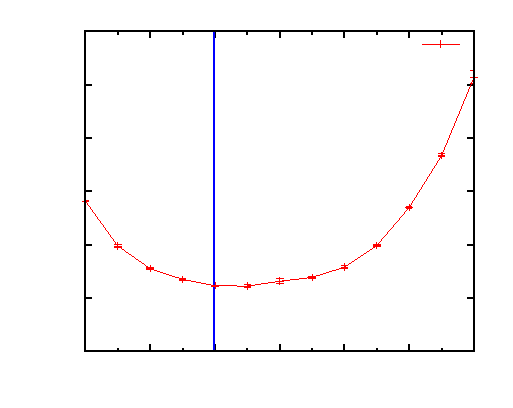
\includegraphics{PrecomputedRankBlockSizeVaryN_6_Rank_WallTime}}%
    \gplfronttext
  \end{picture}%
\endgroup
}
	\caption{$n = 10^6$}
\end{subfigure}

\begin{subfigure}{0.48\textwidth}
	\scalebox{.5}{% GNUPLOT: LaTeX picture with Postscript
\begingroup
  \makeatletter
  \providecommand\color[2][]{%
    \GenericError{(gnuplot) \space\space\space\@spaces}{%
      Package color not loaded in conjunction with
      terminal option `colourtext'%
    }{See the gnuplot documentation for explanation.%
    }{Either use 'blacktext' in gnuplot or load the package
      color.sty in LaTeX.}%
    \renewcommand\color[2][]{}%
  }%
  \providecommand\includegraphics[2][]{%
    \GenericError{(gnuplot) \space\space\space\@spaces}{%
      Package graphicx or graphics not loaded%
    }{See the gnuplot documentation for explanation.%
    }{The gnuplot epslatex terminal needs graphicx.sty or graphics.sty.}%
    \renewcommand\includegraphics[2][]{}%
  }%
  \providecommand\rotatebox[2]{#2}%
  \@ifundefined{ifGPcolor}{%
    \newif\ifGPcolor
    \GPcolortrue
  }{}%
  \@ifundefined{ifGPblacktext}{%
    \newif\ifGPblacktext
    \GPblacktexttrue
  }{}%
  % define a \g@addto@macro without @ in the name:
  \let\gplgaddtomacro\g@addto@macro
  % define empty templates for all commands taking text:
  \gdef\gplbacktext{}%
  \gdef\gplfronttext{}%
  \makeatother
  \ifGPblacktext
    % no textcolor at all
    \def\colorrgb#1{}%
    \def\colorgray#1{}%
  \else
    % gray or color?
    \ifGPcolor
      \def\colorrgb#1{\color[rgb]{#1}}%
      \def\colorgray#1{\color[gray]{#1}}%
      \expandafter\def\csname LTw\endcsname{\color{white}}%
      \expandafter\def\csname LTb\endcsname{\color{black}}%
      \expandafter\def\csname LTa\endcsname{\color{black}}%
      \expandafter\def\csname LT0\endcsname{\color[rgb]{1,0,0}}%
      \expandafter\def\csname LT1\endcsname{\color[rgb]{0,1,0}}%
      \expandafter\def\csname LT2\endcsname{\color[rgb]{0,0,1}}%
      \expandafter\def\csname LT3\endcsname{\color[rgb]{1,0,1}}%
      \expandafter\def\csname LT4\endcsname{\color[rgb]{0,1,1}}%
      \expandafter\def\csname LT5\endcsname{\color[rgb]{1,1,0}}%
      \expandafter\def\csname LT6\endcsname{\color[rgb]{0,0,0}}%
      \expandafter\def\csname LT7\endcsname{\color[rgb]{1,0.3,0}}%
      \expandafter\def\csname LT8\endcsname{\color[rgb]{0.5,0.5,0.5}}%
    \else
      % gray
      \def\colorrgb#1{\color{black}}%
      \def\colorgray#1{\color[gray]{#1}}%
      \expandafter\def\csname LTw\endcsname{\color{white}}%
      \expandafter\def\csname LTb\endcsname{\color{black}}%
      \expandafter\def\csname LTa\endcsname{\color{black}}%
      \expandafter\def\csname LT0\endcsname{\color{black}}%
      \expandafter\def\csname LT1\endcsname{\color{black}}%
      \expandafter\def\csname LT2\endcsname{\color{black}}%
      \expandafter\def\csname LT3\endcsname{\color{black}}%
      \expandafter\def\csname LT4\endcsname{\color{black}}%
      \expandafter\def\csname LT5\endcsname{\color{black}}%
      \expandafter\def\csname LT6\endcsname{\color{black}}%
      \expandafter\def\csname LT7\endcsname{\color{black}}%
      \expandafter\def\csname LT8\endcsname{\color{black}}%
    \fi
  \fi
  \setlength{\unitlength}{0.0500bp}%
  \begin{picture}(4608.00,3600.00)%
    \gplgaddtomacro\gplbacktext{%
      \csname LTb\endcsname%
      \put(660,384){\makebox(0,0)[r]{\strut{} 0}}%
      \put(660,691){\makebox(0,0)[r]{\strut{} 2000}}%
      \put(660,998){\makebox(0,0)[r]{\strut{} 4000}}%
      \put(660,1305){\makebox(0,0)[r]{\strut{} 6000}}%
      \put(660,1612){\makebox(0,0)[r]{\strut{} 8000}}%
      \put(660,1920){\makebox(0,0)[r]{\strut{} 10000}}%
      \put(660,2227){\makebox(0,0)[r]{\strut{} 12000}}%
      \put(660,2534){\makebox(0,0)[r]{\strut{} 14000}}%
      \put(660,2841){\makebox(0,0)[r]{\strut{} 16000}}%
      \put(660,3148){\makebox(0,0)[r]{\strut{} 18000}}%
      \put(660,3455){\makebox(0,0)[r]{\strut{} 20000}}%
      \put(732,264){\makebox(0,0){\strut{}$2^{6}$}}%
      \put(1342,264){\makebox(0,0){\strut{}$2^{8}$}}%
      \put(1952,264){\makebox(0,0){\strut{}$2^{10}$}}%
      \put(2562,264){\makebox(0,0){\strut{}$2^{12}$}}%
      \put(3171,264){\makebox(0,0){\strut{}$2^{14}$}}%
      \put(3781,264){\makebox(0,0){\strut{}$2^{16}$}}%
      \put(4391,264){\makebox(0,0){\strut{}$2^{18}$}}%
      \put(96,1919){\rotatebox{-270}{\makebox(0,0){\strut{}Wall Time ($\mu s$)}}}%
      \put(2561,84){\makebox(0,0){\strut{}Block Size (bits)}}%
    }%
    \gplgaddtomacro\gplfronttext{%
      \csname LTb\endcsname%
      \put(3824,3332){\makebox(0,0)[r]{\strut{}UnalignedNaive}}%
    }%
    \gplbacktext
    \put(0,0){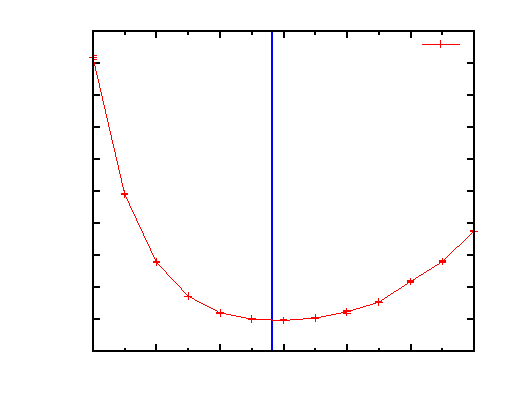
\includegraphics{PrecomputedRankBlockSizeVaryN_7_Rank_WallTime}}%
    \gplfronttext
  \end{picture}%
\endgroup
}
	\caption{$n = 10^7$}
\end{subfigure}
\hfill	
\begin{subfigure}{0.48\textwidth}
	\scalebox{.5}{% GNUPLOT: LaTeX picture with Postscript
\begingroup
  \makeatletter
  \providecommand\color[2][]{%
    \GenericError{(gnuplot) \space\space\space\@spaces}{%
      Package color not loaded in conjunction with
      terminal option `colourtext'%
    }{See the gnuplot documentation for explanation.%
    }{Either use 'blacktext' in gnuplot or load the package
      color.sty in LaTeX.}%
    \renewcommand\color[2][]{}%
  }%
  \providecommand\includegraphics[2][]{%
    \GenericError{(gnuplot) \space\space\space\@spaces}{%
      Package graphicx or graphics not loaded%
    }{See the gnuplot documentation for explanation.%
    }{The gnuplot epslatex terminal needs graphicx.sty or graphics.sty.}%
    \renewcommand\includegraphics[2][]{}%
  }%
  \providecommand\rotatebox[2]{#2}%
  \@ifundefined{ifGPcolor}{%
    \newif\ifGPcolor
    \GPcolortrue
  }{}%
  \@ifundefined{ifGPblacktext}{%
    \newif\ifGPblacktext
    \GPblacktexttrue
  }{}%
  % define a \g@addto@macro without @ in the name:
  \let\gplgaddtomacro\g@addto@macro
  % define empty templates for all commands taking text:
  \gdef\gplbacktext{}%
  \gdef\gplfronttext{}%
  \makeatother
  \ifGPblacktext
    % no textcolor at all
    \def\colorrgb#1{}%
    \def\colorgray#1{}%
  \else
    % gray or color?
    \ifGPcolor
      \def\colorrgb#1{\color[rgb]{#1}}%
      \def\colorgray#1{\color[gray]{#1}}%
      \expandafter\def\csname LTw\endcsname{\color{white}}%
      \expandafter\def\csname LTb\endcsname{\color{black}}%
      \expandafter\def\csname LTa\endcsname{\color{black}}%
      \expandafter\def\csname LT0\endcsname{\color[rgb]{1,0,0}}%
      \expandafter\def\csname LT1\endcsname{\color[rgb]{0,1,0}}%
      \expandafter\def\csname LT2\endcsname{\color[rgb]{0,0,1}}%
      \expandafter\def\csname LT3\endcsname{\color[rgb]{1,0,1}}%
      \expandafter\def\csname LT4\endcsname{\color[rgb]{0,1,1}}%
      \expandafter\def\csname LT5\endcsname{\color[rgb]{1,1,0}}%
      \expandafter\def\csname LT6\endcsname{\color[rgb]{0,0,0}}%
      \expandafter\def\csname LT7\endcsname{\color[rgb]{1,0.3,0}}%
      \expandafter\def\csname LT8\endcsname{\color[rgb]{0.5,0.5,0.5}}%
    \else
      % gray
      \def\colorrgb#1{\color{black}}%
      \def\colorgray#1{\color[gray]{#1}}%
      \expandafter\def\csname LTw\endcsname{\color{white}}%
      \expandafter\def\csname LTb\endcsname{\color{black}}%
      \expandafter\def\csname LTa\endcsname{\color{black}}%
      \expandafter\def\csname LT0\endcsname{\color{black}}%
      \expandafter\def\csname LT1\endcsname{\color{black}}%
      \expandafter\def\csname LT2\endcsname{\color{black}}%
      \expandafter\def\csname LT3\endcsname{\color{black}}%
      \expandafter\def\csname LT4\endcsname{\color{black}}%
      \expandafter\def\csname LT5\endcsname{\color{black}}%
      \expandafter\def\csname LT6\endcsname{\color{black}}%
      \expandafter\def\csname LT7\endcsname{\color{black}}%
      \expandafter\def\csname LT8\endcsname{\color{black}}%
    \fi
  \fi
  \setlength{\unitlength}{0.0500bp}%
  \begin{picture}(4608.00,3600.00)%
    \gplgaddtomacro\gplbacktext{%
      \csname LTb\endcsname%
      \put(732,384){\makebox(0,0)[r]{\strut{} 0}}%
      \put(732,998){\makebox(0,0)[r]{\strut{} 50000}}%
      \put(732,1612){\makebox(0,0)[r]{\strut{} 100000}}%
      \put(732,2227){\makebox(0,0)[r]{\strut{} 150000}}%
      \put(732,2841){\makebox(0,0)[r]{\strut{} 200000}}%
      \put(732,3455){\makebox(0,0)[r]{\strut{} 250000}}%
      \put(804,264){\makebox(0,0){\strut{} 10}}%
      \put(1521,264){\makebox(0,0){\strut{} 100}}%
      \put(2239,264){\makebox(0,0){\strut{} 1000}}%
      \put(2956,264){\makebox(0,0){\strut{} 10000}}%
      \put(3674,264){\makebox(0,0){\strut{} 100000}}%
      \put(4391,264){\makebox(0,0){\strut{} 1e+06}}%
      \put(96,1919){\rotatebox{-270}{\makebox(0,0){\strut{}Wall Time ($\mu s$)}}}%
      \put(2597,84){\makebox(0,0){\strut{}Block Size (bits)}}%
    }%
    \gplgaddtomacro\gplfronttext{%
      \csname LTb\endcsname%
      \put(3824,3332){\makebox(0,0)[r]{\strut{}UnalignedNaive}}%
    }%
    \gplbacktext
    \put(0,0){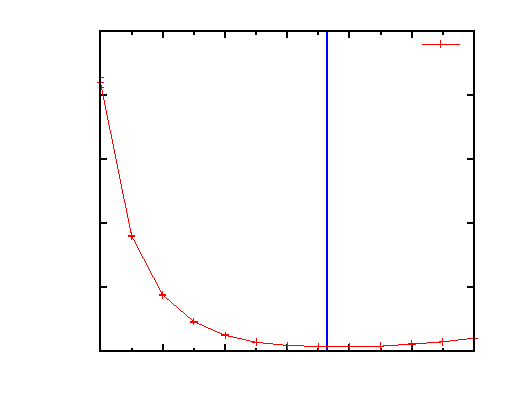
\includegraphics{PrecomputedRankBlockSizeVaryN_8_Rank_WallTime}}%
    \gplfronttext
  \end{picture}%
\endgroup
}
	\caption{$n = 10^8$}
\end{subfigure}
\end{figure}
\end{frame}


\begin{frame}
\frametitle{Experiments}
\begin{itemize}
\item
\end{itemize}
\end{frame}

%----------------------------------------------------------------------------------------

\begin{frame}
\Huge{\centerline{The End}}
\end{frame}

%----------------------------------------------------------------------------------------

\end{document} 